\documentclass[
master=false,
field=inf,
encoding=utf8,
language=czech,
printversion=false,]{kidiplom}

\definecolor{funkcionalni}{RGB}{0,0,100}
\definecolor{pojmenovan}{RGB}{0,100,0}
\definecolor{vedlejsi}{RGB}{100,0,0}
\definecolor{matematicke}{RGB}{100,0,50}
\definecolor{moje}{RGB}{0,50,50}
\definecolor{lightlightgray}{gray}{.875}
\definecolor{lightpink}{RGB}{255,233,233}
\definecolor{obarvi}{RGB}{59,55,20}
\definecolor{lightlightblue}{RGB}{245,251,255}
\newcounter{lispcodecnt}

\setcounter{section}{-1}

\declaretheoremstyle[
headfont=\normalfont\bfseries,
notebraces={(}{)},
headpunct={:}]{mystyle}

\declaretheorem[name=Lispový kód, style=mystyle]{lispcodethm}

\newenvironment{lispcode}[2]
{\def\firstarg{#1}
\def\secondarg{#2}
\VerbatimEnvironment
\begin{mdframed}[backgroundcolor=lightlightgray]
\begin{Verbatim}[commandchars=\\\{\}, numbers=left]}
{\end{Verbatim}
\end{mdframed}
%\vspace{-.92\baselineskip}
\begin{center}
\noindent\begin{minipage}[c]{.9\linewidth}
\begin{lispcodethm}[\firstarg]
\textit{\secondarg}
\end{lispcodethm}
\end{minipage}
\end{center}}

\declaretheorem[name=Lispový test, style=mystyle]{lispcodetest}

\newenvironment{myfigure}[1]{\begin{figure}[#1]\begin{mdframed}[backgroundcolor=lightlightblue,innertopmargin=-2.5pt,innerbottommargin=2.5pt]}{\end{mdframed}\end{figure}}

\newenvironment{myremark}[1]{\begin{remark}[#1]}{\hfill$\blacksquare$\end{remark}}
\newenvironment{myremarkbez}[1]{\begin{remark}[#1]}{\end{remark}}

\newenvironment{lisptest}[2]
{\def\firstarg{#1}
\def\secondarg{#2}
\VerbatimEnvironment
\begin{mdframed}[backgroundcolor=lightlightgray]
\begin{Verbatim}[commandchars=\\\{\}, numbers=left]}
{\end{Verbatim}
\end{mdframed}
%\vspace{-.92\baselineskip}
\begin{center}
\noindent\begin{minipage}[c]{.9\linewidth}
\begin{lispcodetest}[\firstarg]\textit{\secondarg}
\end{lispcodetest}
\end{minipage}
\end{center}}

\title{Přesné výpočty s reálnými čísly}
\title[english]{Precise computation of real numbers}

\author{Ondřej Slavík}
\supervisor{doc. RNDr. Michal Krupka, Ph.D.}

\annotation{Fenomén vyčíslitelnosti reálných čísel provází každého informatika, který se někdy snažil používat počítač k počítání. Jakmile se totiž musíme spolehnout na výpočty s čísly uloženými jako hodnoty, narážíme na limity přesnosti a rozsahu takto reprezentovaných čísel. Řešením není spřesňování pomocí vyšší dotace paměťového prostoru (např. binary32 $\rightarrow$ binary64) a související změna architektury systému, nýbrž fundamentální změna v přístupu k vyčíselní reálných čísel. Tato práce dává návod, jak takovýto přístup přijmout a přináší knihovnu, která základní výpočty a vyčíslení reálných čísel umožňuje.}

\annotation[english]{The Real Numbers' computation phenomenon meets every single computer scientist trying to use computer to compute. When one needs to trust to calculations of numbers saved with their values, the limitations of these numbers' precisivity and range appear. The solution is not to assign more memory (e.g. binary32 $\rightarrow$ binary64) and linked swap of system's architecture but fundamental switch in approach to real numbers' computations. The Work gives a guideline how to admit the access and brings library providing basic real numbers' enumeration and calculation.}

\keywords{reálná čísla, funkce, Lisp, líné vyhodnocování, libovolná přesnost}
\keywords[english]{real numbers, functions, Lisp, lazy evaluation, arbitrary precision}

\thanks{Mockrát děkuji doc. RNDr. Michalu Krupkovi, Ph.D. za vedení práce a rodině za podporu.}

\makeatletter
\AtBeginDocument{%
\@ifpackageloaded{amsthm}%
 {%
  \renewrobustcmd\mdf@patchamsthm{%
   \chardef\kludge@catcode@hyphen=\catcode`\-
   \catcode`\-=12
   \let\mdf@deferred@thm@head\deferred@thm@head
   \pretocmd{\deferred@thm@head}{\@inlabelfalse}%
      {\mdf@PackageInfo{mdframed detected package amsthm ^^J%
                        changed the theorem header of amsthm\MessageBreak}%
      }{%
       \mdf@PackageError{mdframed detected package amsthm ^^J%
                         changed the theorem header of amsthm
                         failed\MessageBreak}%
       }%
   \catcode`\-=\kludge@catcode@hyphen
     }%
 }{}%
}
\makeatother

\newcommand{\mypart}{\newpage\part}

\begin{document}
\setcounter{tocdepth}{3}
\maketitle
\section{Úvod}
Funkcionální programování umožňuje důsledně popsat matematický svět, což bude v této práci ukázáno na příkladu výpočtů reálných čísel. Jako funkcionální jazyk byl zvolen Common Lisp (Lisp) pro jeho syntaktickou jednoduchost, výstižnost a lenost. Každý Lispový kód následuje vždy za matematickým výrazem a ve stejném znění ho převádí. Lisp představuje nástroj, pomocí něhož realizujeme matematické výpočty, hlavním těžištěm poznání je ale vybudovaná matematická teorie, která není specifická pro konkrétní programovací jazyk.

V první části je teoreticky popsáno, co čísla jsou a jak se rozvrstvují podle vlastností na obory. Také je zde ukázáno, jak se s čísly operuje a je představen pojem zobrazení a jeho dva důležité typy -- funkce a posloupnost. Je zde zavedena stěžejní představa, co znamená přesná reprezentace čísla pro jeho různé podoby a představeno několik existujících knihoven.

Ve druhé části práce je popsána konstrukce knihovny \texttt{tnums} přesně vyčíslující reálná čísla. Je využita existence racionálních čísel v Lispu a přidáno Ludolfovo číslo. Zavedená čísla jsou poté kombinována operacemi a měněna svými funkcemi, v návaznosti na to je zavedeno Eulerovo číslo.

V závěrečné části je uvedeno praktické užití řešení a vymezen pojem uživatelské funkce. Je zde ukázáno, jak lze takové funkce přidávat. Také doplníme poslední konstantu, a to Zlatý řez. V poslední kapitole jsou představeny nápady na urychlení a rozšíření práce knihovny \texttt{tnums} a její problémy.

\section*{Značení}
\begin{tabular}{l|l}
$\square$ & konec důkazu \\
$\blacksquare$ & konec poznámky \\
modré pozadí & obrázek \\
nachové pozadí & tabulka \\
$(a,b)$& otevřený interval mezi $a$ a $b$ \\
$[a,b]$ & uzavřený interval mezi $a$ a $b$ \\
$\rightarrow$ & logická implikace nebo \uv{do} \\
$\leftrightarrow$ & logická ekvivalence \\
$\Leftrightarrow$ & \uv{právě tehdy, když} \\
$\cup$& množinové sjednocení \\
$\cap$ & množinový průnik \\
$|a|$ & absolutní hodnota čísla $a$ \\
:= & přiřazení \\
$\frac{d}{dx}f(x_0)$ & derivace funkce $f$ v bodě $x_0$; je-li jasná proměnná, pak jen $f^{'}(x)$
\end{tabular}
\mypart{Teorie}
V teoretické části se podíváme na axiomatickou teorii množin a poté naznačíme, jak se z ní dají vytvořit čísla. Zjistíme, že čísla jsou množinami. Poté se stručně podíváme na matematické operace a matematické funkce. Zjistíme, že jakékoli číslo lze vyjádřit jako funkci a že funkce je také množina. Poté se zaměříme na uložení čísla v paměti počítače, která je z fyzikální podstaty konečná. Nejprve jako intelektuální cvičení a poté jako reálně existující knihovny.
\section{Čísla}
Číslo je matematický objekt, který na intuitivní úrovni všichni chápeme. To znamená, že každý dokáže o libovolném objektu říci, zda se jedná o číslo, nebo nikoli, a všichni se na tom shodneme. Je číslem $3$? Je číslem $2.999\ldots$? Je číslem $e$? 

Vágní pokus o definici by mohl vypadat tak jako na české wikipedii:

\begin{definition}[Číslo -- naivní \cite{wiki:cislo}]
Číslo je abstraktní entita užívaná pro vyjádření množství nebo pořadí.
\end{definition}

Uvedená definice přiřazuje číslům dvě funkce -- kardinální a ordinální. Jinak o povaze čísel neříká mnoho. Víme, že je to abstraktní entita -- to znamená, že ji nelze zapsat samu o sobě, ale je třeba použít nějaký symbol. Symbolem reprezentujícím číslo tři je $3$, $\frac{6}{2}$ nebo třeba i $2.999\ldots$. Symbolický zápis čísla zřejmě není jednoznačný. $3$ není to samé jako $2.999\ldots$, ale číslo $3$ je to samé jako číslo $2.999\ldots$. Z toho plyne, že symbol s referencí na nějakou entitu a tato entita samotná se od sebe liší. Alenka takhle zjistila rozdíl mezi tím, jak se říká názvu písně, jaké je její jméno, jak se píseň jmenuje a co píseň opravdu je \cite{TtLG}. Známe-li rozdíl mezi koncepty čísla a symbolu, který ho repreznetuje, je možné využít pro reprezentaci čísel i jiné symboly než číslice jako jsou například písmena či složené matematické výrazy -- například $e = \lim_{n \to \infty} \left(1 +\frac{1}{n} \right)^n = \sum_{n\in\mathbb{N}}\frac{1}{n!}$.

Číslo je tedy charakterizováno nikoli svým zápisem, ale svým obsahem. Tato vlastnost je společná s jinými matematickými objekty -- s množinami. Množina je také dána svým obsahem, nikoli svým zápisem (této vlastnosti se říká princip extenzionality). Například $\{0, 1, 2, 3 \} = \{ n | n \in \mathbb{N} \land n \leq 3 \}$ je stejná množina zapsaná dvěma různými způsoby. Symbol \uv{$=$} je tedy ekvivalence na hodnotách.

\subsection{Přirozená čísla}
Přirozená čísla jsou čísla, jejichž \textit{kardinalita} určuje počet nedělitelných částí celku. Historicky asi vznikla nejdříve, proto se nazývají přirozená (anglicky \textit{natural} -- přírodní). Jedná se o čísla nula, jedna, dva, atd. Běžnými symboly těchto čísel jsou 0, 1, 2, atd. Vlastností přirozených čísel je, že \textit{každé} číslo $n$ má následníka. Toho značíme $s(n)$ nebo $n+1$ \cite{LambdaCalcul}.

Hodnota přirozeného čísla je počet entit v nějakém souboru -- například počet krav ve stádu, počet prstů na ruce, nebo počet třešniček na dortu. \textit{Následník} takového čísla značí, kolik entit bude v souboru, pokud se do stáda narodí další kráva, na ruku se přišije jeden prst nebo je do krému přidána další třešnička.

I přirozená čísla jsou \textit{množiny}. Konkrétně v~tomto textu je zavedu v Zermelově-Fraenkelově (ZF) axiomatici teorii množin. Je snadné nahlédnout, že stačí zkonstruovat číslo nula a \textit{zobrazení} $s$ přiřazující každému číslu následníka. Poté budeme mít celou nekonečnou množinu přirozených čísel zkonstruovanou. Protože se jedná o výklad teorie množin, celý zbytek této podkapitoly je pouze velmi stručný výtah z \cite{TeMno}.

Definice přirozených čísel je induktivní a stojí na jednoduché myšlence Johna von Neumanna, že \uv{přirozené číslo je množina všech menších přirozených čísel}. Číslo nula je zde prázdná množina značená $0$, $\emptyset$ nebo $\{ \}$. Následník čísla je sjednocení čísla s množinou obsahující toto číslo, čili $s(n) = n \cup \{n\}$.

Několik nejmenších přirozených čísel vypadá tedy následovně.
\begin{example}[Nejnižší přirozená čísla coby množiny]
\begin{equation}
0 = \emptyset
\end{equation}
\begin{equation}
1 = s(0) = 0 \cup \{ 0 \} = \emptyset \cup \{ \emptyset \} = \{ \emptyset \}
\end{equation}
\begin{equation}
2 = s(1)= 1 \cup \{ 1 \} = \{ \emptyset \} \cup \{ \{ \emptyset \} \} = \{ \emptyset , \{ \emptyset \} \}
\end{equation}
\begin{equation}
3 = s(2)= 2 \cup \{ 2 \} = \{ \emptyset , \{ \emptyset \} \} \cup \{ \{ \emptyset , \{ \emptyset \} \} \} = \{ \emptyset , \{ \emptyset \} , \{ \emptyset , \{ \emptyset \} \} \} 
\end{equation}
\begin{equation}
\begin{split}
4 =s(3)= 3 \cup \{ 3 \} = \{ \emptyset , \{ \emptyset \} , \{ \emptyset , \{ \emptyset \} \} \}  \cup \{ \{ \emptyset , \{ \emptyset \} , \{ \emptyset , \{ \emptyset \} \} \}  \} = \\ = \{ \emptyset , \{ \emptyset \} , \{ \emptyset , \{ \emptyset \} \} , \{ \emptyset , \{ \emptyset \} , \{ \emptyset , \{ \emptyset \} \} \}  \}
\end{split}
\end{equation}
\end{example}

\begin{myremark}{Provázání hodnot a podmnožin}\label{pozn:kard_podm}
Všimněme si, že kardinalita v tomto pojetí znamená počet podmnožin, neboli číslo $n$ má $n$ podmnožin. Tím se provázaly dva zdánlivě cizí pojmy a sice \textit{podmnožinovost} a \textit{hodnota} čísla. V tomto kontextu pak není překvapivá podobnost srovnávacích symbolů $\subseteq$ a $\leq$.
\end{myremark}

Zermelova-Fraenkelova teorie stojí na následujících pěti axiomech a jednom axiomovém schématu (někdy uváděno jako 6 axiomů).

\begin{itemize}
\item Axiom extenzionality: $(\forall u)((u \in x \leftrightarrow u \in y) \rightarrow x = y)$
\item Axiom fundovanosti: $ (\forall a)(a \neq \emptyset \rightarrow (\exists x)(x \in a \land x \cap a = \emptyset))$
\item Axiom sumy: $(\forall a)(\forall b)(\exists z)(\forall x)(x \in z \leftrightarrow (x = a \lor x = b))$
\item Axiom potence: $(\forall a)(\exists z)(\forall x)(x \in z \leftrightarrow x \subset a)$
\item Axiom nekonečna: $(\exists z)(\emptyset \in z \land (\forall x)(x \in z \rightarrow x \cup \{ x \} \in z))$
\item Schéma axiomů nahrazení: Je-li $\Psi (u, v)$ formule, která neobsahuje volné proměnné $w$ a $z$, potom formule $$\begin{aligned}(\forall u)(\forall v)(\forall w)((\Psi (u,v) \land \Psi (u, w)) \rightarrow v = w) \rightarrow \\ \rightarrow (\forall a)(\exists z)(\forall v)(v \in z \leftrightarrow (\exists u)(u \in a \land \Psi (u,v))) \end{aligned}$$ je axiom nahrazení.
\end{itemize}

Z těchto axiomů je možné odvodit i (slabší) tvrzení, která se někdy přijímají jako axiomy a sice
\begin{itemize}
\item Axiom dvojice: $(\forall a)(\forall b)(\exists z)(\forall x)(x \in z \leftrightarrow (x = a \lor x = b))$
\item Schéma axiomů vydělení: Je-li $\varphi (x)$ formule, která neobsahuje volnou proměnnou $z$, potom formule $(\forall a)(\exists z)(\forall x)(x \in z \leftrightarrow  (x \in a \land \varphi (x)))$ je axiom vydělení.
\end{itemize}

Z axiomů ZF je pro naše zkoumání důležitý například axiom nekonečna -- existuje alespoň jedna (nekonečná) množina. Za pomoci dalších axiomů poté konstruujeme další prvky, jako třeba prázdnou množinu -- tu dostaneme pomocí axiomu vydělení s jakoukoli množinou $a$ a formulí $\varphi(x) = x \neq x$ -- prázdná množina je tedy $\emptyset = \{ x | x \in a \land x \neq x \}$. Dále získáváme, že sjednocení množin je také množina, podobně jejich průnik.

\begin{definition}[Induktivní množina]
Množina $A$ je \textit{induktivní}, pokud platí $(\emptyset \in A) \land (\forall a \in A)((a \cup \{ a \}) \in A)$.
\end{definition}

\begin{definition}[Přirozená čísla]
\begin{equation}
\mathbb{N} = \bigcap \{A | A \text{~je induktivní} \}
\end{equation}
\end{definition}

Množina přirozených čísel je nejmenší induktivní množina a je podmnožinou každé induktivní množiny. $\mathbb{N}$ je nejmenší nekonečný \textit{kardinál} a také jediný \textit{spočetný} kardinál.

\begin{myremark}{Značení přirozených čísel}
Množina $z$ v axiomu nekonečna je stejná množina jako $\mathbb{N}$. V teorii množin se značí $\omega$, při zkoumání kardinality pak $\aleph_0$. Pro označení přirozených čísel bez nuly zaveďme horní index $+$ ($\mathbb{N^+} = \mathbb{N} - \{0\}$).
\end{myremark}

\begin{myremark}{Nula je přirozená}
Z definice přirozených čísel podle ZF přímo vyplývá, že součástí přirozených čísel je i číslo nula. Dle mého i stádo, ve kterém není žádná kráva, je stále stádem; ruka bez prstů je stále rukou; dort bez třešniček je i tak dort.\end{myremark}

\subsection{Vyšší obory čísel}
\label{kap:vyssi_obory_cisel}
Vyšším oborem čísel jsou čísla celá, značená $\mathbb{Z}$, a jsou to všechna čísla, která mohou vzniknout libovolným odčítáním přirozených čísel. Jejich výčet je diskrétní: $\mathbb{Z} = \{0, 1, -1, 2, -2, \ldots\}$\cite{OEIS:integer}. Zde \uv{$-$} je znaménko odčítání (snížení hodnoty prvního argumentu o hodnotu druhého).

Další číselný obor jsou čísla racionální, pro která se vžilo označení $\mathbb{Q}$ a racionálním číslem je číslo $x$, pokud jde zapsat jako $y/z$, kde $y \in \mathbb{Z}$ a $z \in \left( \mathbb{Z} \setminus \{0\} \right)$ a \uv{$/$} je symbol operace dělení \cite{SPIVAK:calculus}. Množina racionálních čísel je spočetná, $\mathbb{Q} = \{0, 1, 1/2, -1, 1/3, -1/2, 2, 1/4, \ldots \}$.

Po zavedení racionálních čísel stále v budovaném číselném systému nemáme například délku úhlopříčky jednotkového čtverce -- takovéto číslo značíme $\sqrt{2}$ -- nebo třeba poměr obvodu kružnice k jejímu průměru -- toto značíme $\pi$. Když do systému doplníme všechna tato čísla, získáváme tzv. číselnou osu (přímku) reprezentující čísla reálná, značená $\mathbb{R}$. Množině přidaných čísel říkáme iracionální (nejsou racionální) a značíme ji $\mathbb{I}$, $\mathbb{I} = \mathbb{R} \setminus \mathbb{Q}$ \cite{tabulky}. Ke každým dvěma reálným číslům $r$ a $\varepsilon$ lze najít racionální číslo $q$ tak, aby
\begin{equation}\label{rov:rac_u_real}
|r-q|\leq\varepsilon \text{~\cite{TeCis}}.
\end{equation}

V množině reálných čísel matematikové objevili ještě jemnější struktury, než je dělení na obory, které jsem teď představil. První jmenované iracionální číslo $\sqrt{2}$ je tzv. \textit{algebraické}, protože může vypadnout jako řešení nějaké algebraické rovnice, např. $x ^ 2 = 2$ nebo $(-x) ^ 2 = 2$, zatímco druhé jmenované -- tzv. \textit{Ludolfovo číslo} ($\pi$) -- takovouto vlastností nedisponuje, je \textit{nealgebraické} (též \textit{transcendentní}) \cite{TeMno}. Dále v oboru reálných čísel existují tzv. \textit{rekurzivní čísla} (\textit{computable reals} -- vizte kapitolu \ref{kap:computable-reals}), která se dají vyčíslit v konečném čase. Pro reálné číslo $r$ a dané $\varepsilon$ existuje vyčíslitelná funkce (pro konečný vstup někdy skončí), jejímž výsledkem je racionální číslo $q$ tak, že platí nerovnice \ref{rov:rac_u_real}. Ostatní čísla jsou \textit{nerekurzivní} a protože Turingových strojů je spočetně mnoho, je nerekurzivních čísel nespočetně mnoho \cite{wiki:CompN}. Přechod od racionálních čísel k rekurzivním, kterým se zabývá tato práce, je velmi složitý. V jednom oboru jsou i složité věci vcelku jednoduché, zatímco v tom druhém jsou i jednoduché věci vceklu složité.

Vyššími obory jsou strukturovaná čísla -- uvažujeme více číselných os a číslo má $2^n$ složek. Jedná se o komplexní čísla ($\mathbb{C}, n = 1$), kvaterniony ($\mathbb{H}, n = 2$), oktoniony ($\mathbb{O}, n = 3$) -- těmto čtyřem (společně s reálnými čísly) oborům říkáme \textit{normované algebry s dělením} (\textit{normed division algebra}) \cite{DAaQT}. Existují ještě vyšší obory (sedeniony -- $\mathbb{S}, n = 4$ atd.), tato práce se nicméně dále zabývá pouze jednorozměrnými čísly a v dalším textu je \uv{číslem} myšleno číslo \textit{reálné}.

\subsection{Operace s čísly}
\label{operace_s_cisly}
Již v kapitole \ref{kap:vyssi_obory_cisel} byly zmíněny 3 operace -- \textit{odčítání} (rozdíl), \textit{dělení} (podíl) a \textit{odmocňování} (odmocnina). K nim existují ještě operace opačné, a ty po řadě nazýváme \textit{sčítání} (součet), \textit{násobení} (součin) a \textit{umocňování} (mocnina).

Binární operace se značí znaménkem mezi operandy. Například součet čísel $x$ a $y$ značíme $x+y$ atd. Základní značení operací je uvedeno v~tabulce \ref{tab:znamenka_operaci}. Binárním operacím, které mají jako první operand neutrální prvek (při operaci s číslem je výsledkem toto číslo), budeme říkat unární. Unárními operacemi je číslo opačné (k číslu $x$ je opak číslo $0-x$ a značíme ho $-x$) a převrácené číslo (k číslu $x\neq0$ je číslen převráceným číslo $1/x$ a značíme ho $/x$ nebo $x^{-1}$).

Operacím $\langle +, -\rangle$ říkáme aditivní, $\langle *, /\rangle$ multiplikativní a $\langle\string^ , \surd\rangle$ mocninné. Operace v uvedených dvojicích jsou příbuzné, příslušné vztahy nazveme \uv{horizontální}. Mezi operacemi však existují též vztahy \uv{vertikální}. Platí
\begin{equation}
x*n = \underbrace{x + x + \ldots + x}_{n\text{-krát}} \text{~a také~} x^n = \underbrace{x * x * \ldots * x}_{n\text{-krát}}.
\end{equation}
Máme tedy návod, jak teoreticky vytvořit více operací.

Další operace je daná předpisem
\begin{equation}
x\#n = \underbrace{x \string^ x \string^ \ldots \string^ x}_{n\text{-krát}}
\end{equation}
a nazýváme ji tetrace \cite{Operations}.

Pro operace vyšší arity je pak zvykem používat prefixovou notaci jednoho velkého znaménka -- součet $a_0 + a_1 + a_2$ je pak zapsán jako $\scalerel*{+}{\sum}(a_0, a_1, a_2)$ nebo též $\sum_{i=0}^2(a_i)$. Součin $a_0 * a_1 * a_2$ pak $\scalerel*{*}{\sum}(a_0, a_1, a_2)$ nebo $\prod_{i=0}^2(a_i)$.

\begin{table}[H]
\begin{mdframed}[backgroundcolor=lightpink,innertopmargin=-2.5pt,innerbottommargin=2.5pt]
\centering
\caption{Symboly operací s čísly}
\begin{tabular}{|>{\columncolor[gray]{1}}r|>{\columncolor[gray]{1}}l|}
\hline
Operace & Značení \\ \hline \hline
sčítání & $x+y$ \\
odčítání & $x-y$ \\
násobení & $x*y$, $x\cdot y$ nebo $xy$\\
dělení & $x/y$ nebo $\frac{x}{y}$ \\
umocňování & $x^y$ nebo $x\string^ y$\\ 
odmocňování & $\sqrt[y]{x}$ \\\hline
\end{tabular}\label{tab:znamenka_operaci}

Tabulka zobrazuje zápis binárních operací s čísly $x$ a $y$.
\end{mdframed}
\end{table}

\subsection{Funkce čísel}
\label{funkce_cisel}
Další manipulace s čísly jsou tzv. funkce, které si představujeme jako nekonečnou tabulku o dvou sloupcích, které představují výstupní a výstupní hodnoty (v tabulce \ref{tab:sinus_input_output} jsou uvedeny některé hodnoty pro funkci sinus). V informatice též mluvíme o argumentu funkce a návratové hodnotě. Příklady funkcí jsou funkce \textit{goniometrické}, funkce \textit{exponenciální} či \textit{logaritmus}.

\begin{table}[H]
\begin{mdframed}[backgroundcolor=lightpink,innertopmargin=-2.5pt,innerbottommargin=2.5pt]
\centering
\caption{Nekonečná vstupně/výstupní tabulka funkce $sinus$}
\label{tab:sinus_input_output}
\begin{tabular}{|>{\columncolor[gray]{1}}c|>{\columncolor[gray]{1}}c|}
\hline
Vstup & Výstup\\ \hline \hline
$0$ & $0$ \\ 
$1$ & $0.8414709848078965\ldots$ \\
$2$ & $0.9092974268256817\ldots$ \\
$3$ & $0.1411200080598672\ldots$ \\
$4$ & $-0.7568024953079282\ldots$ \\
\multicolumn{2}{|>{\columncolor[gray]{1}}c|}{$\vdots$} \\ \hline
\end{tabular}

Tabulka obsahuje v prvním sloupci vstupní hodnoty funkce sinus a ve druhém hodnoty výstupní. Tabulka je nekonečná ve vertikálním směru, v horizontálním jsou pouze dva sloupce -- pro argument a vrácenou hodnotu.
\end{mdframed}
\end{table}

Funkce jsou velmi užitečným a potřebným nástrojem takřka ve všech odvětvích matematiky a jsou často zdrojem \textit{iracionálních} (\textit{transcendentních}) čísel -- například $\mathrm{atan}(1)$ dá za výsledek čtvrtinu \textit{Ludolfova čísla}.

\begin{definition}[Uspořádaná $n$-tice \cite{TeMno}]
Jsou-li dány množiny $a_1,a_2,\ldots a_m$, uspořádanou $n$-tici množin $a_1,a_2,\ldots,a_n$ pro $n<m$ definujeme tak, že pro $n=1$ položíme
\begin{equation}
\langle a_1 \rangle = a_1
\end{equation}
a je-li již definována uspořádaná $n$-tice $\langle a_1, a_2,\ldots , a_n \rangle$, položíme
\begin{equation}
\langle a_1, a_2, \ldots a_{n+1} \rangle = \langle \langle a_1, a_2 \ldots a_n \rangle , a_{n+1} \rangle .
\end{equation}
\end{definition}

\begin{definition}[Kartézský součin \cite{EPJVMAI} \cite{RachALG1}]
Nechť $A_0, A_1, \ldots , A_{n}$ jsou množiny. Symbolem $\bigtimes_{i=0}^{n} A_i$ či $A_0 \times A_1 \times \ldots \times A_{n}$ označujeme množinu všech uspořádaných $(n+1)$-tic tvaru $\langle a_0, a_1, \ldots a_{n} \rangle$, přičemž $(a_0 \in A_0)\land (a_1 \in A_1)\land\ldots\land (a_{n}\in A_{n})$, neboli
\begin{equation}
A_0 \times A_1 \times \ldots \times A_{n} = \{\langle a_0 , a_1, \ldots , a_{n}  \rangle | (\forall i \in \mathbb{N}, i \leq n)(a_i \in A_i)\}
\end{equation}
a tuto množinu nazýváme kartézským součinem množin $A_0, A_1, \ldots A_n$.
\end{definition}

\begin{myremark}{Množinovost kartézského součinu}\label{rem:mnozinovost_KS}
Že je kartézský součin (KS) množina jsem zavedl definitoricky, jako to udělaly autorky v \cite{EPJVMAI}, ovšem nemusí to být úplně jasné, je to ovšem dokazatelné. V \cite{TeMno} se kartézský součin zavádí jako třída (soubor množin, který množina být nemusí -- například třída všech množin množinou není) a poté se pomocí axiomu potence jeho množinovost dokazuje.
\end{myremark}

\begin{definition}[Relace \cite{EPJVMAI}]
Relace mezi množinami $A$ a $B$ je libovolná podmnožina $\mathcal{R}$ kartézského součinu $A\times B$. Je-li $A=B$, mluvíme o relaci na $A$. Náleží-li dvojice $\langle a, b \rangle$ relaci $\mathcal{R}$, t.j. $\langle a,b \rangle \in \mathcal{R}$, říkáme, že $a$ a $b$ jsou v relaci $\mathcal{R}$, a zapisujeme též $a\mathcal{R}b$.
\end{definition}

\begin{definition}[Zobrazení \cite{EPJVMAI}]
Relaci $f \subseteq A \times B$ nazveme \textit{zobrazením} množiny $A$ do množiny $B$, jestliže platí, že ke každému prvku $x \in A$ existuje právě jeden prvek $y \in B$ takový, že $\langle x, y \rangle \in f$.
\end{definition}

Je-li relace $f \subseteq A \times B$ zobrazení, pak skutečnost, že $\langle x, y \rangle \in f$ zapisujemme ve tvaru $y = f(x)$. Rovněž používáme zápis $f:A\rightarrow B$, což znamená, že $f$ je zobrazení $A$ do $B$. Dále $x$ nazýváme \textit{nezávisle proměnnou} a $y$ \textit{závisle proměnnou} \cite{DK:DPFJP}.

\begin{definition}[Reálná posloupnost \cite{EPJVMAI}]
Zobrazení množiny $\mathbb{N}$ do množiny $\mathbb{R}$ nazýváme \textit{reálná posloupnost}.
\end{definition}

Místo obecného značení $a:\mathbb{N}\rightarrow\mathbb{R}$ pro zobrazení se vžilo pro posloupnost značení $\{a_n\}_{n\in\mathbb{N}}$ nebo $\{a_n\}_{n=0}^{\infty}$. Obraz bodu $n$ se značí $a_n$ a říkáme mu také $n$-tý člen posloupnosti $a$ \cite{EPJVMAI}. 

\begin{definition}[Nekonečná číselná řada \cite{ZDVNNR}]
Nechť $\{a\}_{n\in\mathbb{N}}$ je reálná posloupnost. Symbol $\sum_{n\in\mathbb{N}}a_n$ nebo $a_0 + a_1 + a_2 + \ldots$ nazýváme nekonečnou číselnou řadou.
\end{definition}

\begin{definition}[Posloupnost částečných součtů \cite{ZDVNNR}]
Posloupnost $\{s_n^a\}$, kde $s^a_n=\sum_{i=0}^na_i$ nazýváme \textit{posloupnost částečných sou\-čtů} řady $\sum_{n\in\mathbb{N}}a_n$.
\end{definition}

\begin{definition}[Konvergence řady \cite{ZDVNNR}]
Existuje-li vlastní limita $\lim_{n\to\infty}s^a_n = s$, řekneme, že řada $\sum_{n\in\mathbb{N}}a_n$ konverguje a má součet $s$.
\end{definition}

\begin{definition}[Divergence řady \cite{ZDVNNR}]
Neexistuje-li vlastní limita $\lim_{n\to\infty}s^a_n$, řekneme, že řada $\sum_{n\in\mathbb{N}}$ diverguje. Pokud limita $\lim_{n\to\infty}s^a_n$ neexistuje, říkáme, že řada osciluje. Pokud je $\lim_{n\to\infty}s^a_n = \infty$, pak říkáme, že řada diverguje k $\infty$. Pokud je $\lim_{n\to\infty}s^a_n = -\infty$, pak říkáme, že řada diverguje k $-\infty$. 
\end{definition}

\begin{definition}[Zbytek po $n$-tém členu řady \cite{ZDVNNR}]
Nechť $\sum_{n\in\mathbb{N}}a_n$ je konvergentní řada. Její součet $s$ lze psát ve tvaru $s = s_n^a + R_n^a$, kde $s_n^a=\sum_{i=0}^na_i$ je $n$-tý částečný součet řady $\sum_{n\in\mathbb{N}}a_n$ a $R_n^a = \sum_{i=n+1}^{\infty}a_i$ se nazývá \textit{zbytek po $n$-tém členu} a znamená velikost chyby, které se doupouštíme, když místo celé řady posčítáme pouze prvních $n$ členů posloupnosti $\{a_n\}_{n\in\mathbb{N}}$.
\end{definition}

\begin{definition}[Reálná funkce reálné proměnné \cite{DK:DPFJP}]
Buď $M\subseteq R$. Zobrazení $f:M\rightarrow\mathbb{R}$ nazýváme \textit{reálnou funkcí reálné proměnné} nebo stručně \textit{funkcí} jedné proměnné.

Množina $M$ se nazývá \textit{definiční obor} funkce $f$ a značí se $D(f)$, množina $H(f) = \{f(x) | x \in M \}$ se nazývá \textit{obor hodnot} funkce $f$. 
\end{definition}

\begin{example}[Sinus jako zobrazení]
Funkce $y=sin(x)$ je definována pro všechna $x\in\mathbb{R}$ a její obor hodnot je interval $[-1,1]$, jedná se tedy o reálnou funkci reálné proměnné. Pokud budeme hledět jen na obrazy $sin(x), x\in\mathbb{N}$ (jako v tabulce \ref{tab:sinus_input_output}), jedná se o reálnou posloupnost.
\end{example}

Zobrazení $f:A\rightarrow B$ je definováno tak, že $A$ i $B$ jsou množiny. Poznámka \ref{rem:mnozinovost_KS} říká, že je množinou i kartézský součin množin. Tedy lze definovat též zobrazení $\mathbb{R}\times\mathbb{I}\rightarrow\mathbb{Q}\times\mathbb{Z}\times\mathbb{N}$ atp., aniž bychom museli definici zobrazení jakkoli upravovat.

Existují podobnosti mezi operacemi a funkcemi. Pokud se odprostíme od infixové notace a místo $a + b$ napíšeme $+(\langle a, b\rangle)$, lze i operace vyjádřit jako funkce. Matematickou operaci pak chápeme jako speciální případ funkce, $n$-ární reálná operace je funkce $\bigtimes_{i=1}^{n}\mathbb{R}\rightarrow \mathbb{R}$.

Funkce $\emptyset \rightarrow \mathbb{R}$ je konstanta, neboť podle definice zobrazení, pokud jsou v relaci $\langle \emptyset, x\rangle$ a $\langle \emptyset, y\rangle$, pak $x = y$. Funkce se vždy zobrazuje na stejné číslo, a proto se jedná konstantu. Z toho plyne, že funkcemi můžeme modelovat jakákoli čísla i manipulaci s nimi.

\begin{definition}[Mocninná řada \cite{ZDVNNR}]
Buď $\{a_n\}_{n\in\mathbb{N}}$ posloupnost reálných čísel, $x_0$ libovolné reálné číslo. \textit{Mocninnou řadou} se středem v bodě $x_0$ a koeficienty $a_n$ rozumíme řadu ve tvaru
\begin{equation}
a_0+a_1(x-x_0)+a_2(x-x_0)^2+\ldots+a_n(x-x_0)^n+\ldots=\sum_{n\in\mathbb{N}}a_n(x-x_0)^n.
\end{equation}
\end{definition}

\begin{definition}[Taylorova řada \cite{ZDVNNR}]\label{def:taymac_rada}
Nechť funkce $f$ má v bodě $x_0$ derivace všech řádů. Mocninnou řadu ve tvaru $\sum_{n\in\mathbb{N}}\frac{f^{(n)}(x_0)}{n!}(x-x_0)^n$ nazýváme \textit{Taylorovou řadou} funkce $f$ v bodě $x_0$.

Je-li $x_0=0$, mluvíme o \textit{Maclaurinově řadě} funkce $f$ a je ve tvaru $\sum_{n\in\mathbb{N}}\frac{f^{(n)}(0)}{n!}x^n$.

Zbytku po $n$-tém členu Taylorovy řady říkáme $n$-tý Taylorův zbytek a značíme ho $R^{f,a}_n(x)$.
\end{definition}

\begin{definition}[Geometrická řada \cite{ZDVNNR}]
Řadu nazýváme geometrickou, pokud je ve tvaru
\begin{equation}
a + a*q + a*q^2 + a*q^3 +\ldots = \sum_{i\in\mathbb{N}}aq^i
\end{equation}
\end{definition}

\begin{fact}[Částečný součet geometrické řady \cite{ZDVNNR}]\label{vet:o_castecnem_souctu_geometricke_rady}
Pro geometrickou řadu ve tvaru $\sum_{i\in\mathbb{N}}aq^i$ a $|q|<1$ platí
\begin{equation}
s^a_n=\sum_{i=0}^na*q^i=a\frac{1-q^{n+1}}{1-q}
\end{equation}
\end{fact}

\begin{fact}[Geometrická řada]\label{vet:o_geometricke_rade}
Pro geometrickou řadu ve tvaru $\sum_{i\in\mathbb{N}}aq^i$ a $|q|<1$ platí
\begin{equation}
\sum_{i\in\mathbb{N}}aq^i = \frac{a}{1-q}
\end{equation}
\end{fact}

\begin{fact}[Zbytek geometrické řady]\label{vet:o_zbytku_geometricke_rady}
Pro $n$-tý zbytek geometrické řady $\sum_{i\in\mathbb{N}}aq^i$ platí
\begin{equation}
R_n = \frac{aq^{n+1}}{1-q}
\end{equation}
\end{fact}	
\clearpage
\section{Čísla v počítači}
Standardně jsou čísla v počítači uložena jako sled bitů v nějaké reprezentaci vyjadřující hodnotu. Tímto způsobem lze reprezentovat číslo jen s danou přeností a rozsahem, což je však v řadě případů dostačující. Čísla lze reprezentovat i naprosto přesně -- pomocí struktur je reprezentujícími a s nimi manipulujícími. I tyto samozřejmě musí být uloženy v paměti, v tomto případě se však nejedná o uložení hodnoty čísla, nýbrž se ukládá abstrakce, která číslo na požádání umí vygenerovat. Tento přístup nazýváme líným. Nejprve bude popsáno ukládání čísel jako hodnot a na jeho přesnost. Poté navrhneme struktury pro přesná čísla a nakonec budou ukázány existující knihovny.

\subsection{Čísla uložená jako hodnoty}
Paměť počítače většinou pracuje s tzv. \textit{bity}, paměťovými buňkami nabývajícími dvou rozlišitelných hodnot \cite{KepOS}. Ke kódování čísel se tedy používá výhradně dvojková soustava. Celá následující podkapitola pojednávající o uložení čísel jejich hodnotami je převzata z \cite{Knu02}.

\subsubsection{Vážený poziční kód}
Číslo v soustavě o základu $b$ lze dešifrovat následovně:
\begin{equation}
(\ldots a_2a_1a_0.a_{-1}a_{-2} \ldots )_b = \cdots + a_2b^2 + a_1b + a_0 + \frac{a_{-1}}{b} + \frac{a_{-2}}{b^2} + \cdots
\end{equation}kde čísla $a_n$ nazýváme číslice a symbol \uv{$.$} řádovou tečkou -- speciálně pak tečkou \textit{desetinnou} ($b=10$) nebo \textit{dvojkovou} ($b=2$).

\begin{example}[Převod z váženého pozičního kódu]
\begin{equation}
(101010.101)_2 = (42.625)_{10}
\end{equation}
\end{example}

\subsubsection{Záporná čísla}
V případě zápisu čísla váženým pozičním kódem lze strukturu pokrývající i záporná čísla přímočaře vytvořit přidáním příznaku (rozšířit jeho reprezentaci o jeden bit), zda se jedná o číslo kladné či nikoliv. V této reprezentaci lze vyjádřit zápornou i kladnou nulu. Tomutu kódování se říká kód \textit{velikostí a znaménkem (signed-magnitude)}.

Jinou možností je záporná čísla vnímat jako opak čísel kladných i na úrovni reprezentace, čili záporné číslo opačné ke kladnému v binární reprezentaci vypadá jako negace bitů daného kladného čísla. Opět zde vyvstává problém se zápornou nulou. Tomutu kódování se říká \textit{jedničkový doplněk (ones' complement)}.

Když od všech záporných čísel v jedničkovém doplňku odečteme číslo jedna, rozprostřeme čísla efektivně, tj. odpadne problém s dvojí reprezentací nuly. Tomutu kódování se říká \textit{dvojkový doplněk (two's complement)}.

\subsubsection{Plovoucí řádová tečka}
U váženého pozičního kódu známe přesně pozici řádové tečky -- je mezi číslicemi $a_0$ a $a_{-1}$. Alternativním přístupem je kódování s \textit{plovoucí} řádovou tečkou.

Plovoucí číslo je dáno uspořádanou dvojicí $\langle e,f\rangle = f * b^{e-q}$, kde $e$ nazýváme \textit{exponent} a $f$ \textit{zlomkovou částí (fraction)}. Čísla $b$ a $q$ jsou konstanty dané použitým typem, $b$ se nazývá \textit{základ} a $q$ \textit{přesah}.

\begin{example}[Plovoucí číslo -- jednoduchá přesnost]
Číslo s jednoduchou přesností (\textit{single} dle IEEE 754-1985, \textit{binary32} dle IEEE 754-2008) je uloženo v paměti jako 32b struktura. První bit je příznak znaménka, dalších 8 bitů je pro exponent a dalších 23 bitů pro fraction. Konstanty jsou ohodnoceny následovně: $q=127$, $b=2$. V \textit{C}, \textit{C++}, \textit{C\#} nebo \textit{Javě} se tento číselný datový typ nazývá \textit{float}, v \textit{Haskellu Float} a v \textit{Lispu} pak \textit{single-float} \cite{wiki:float}.
\begin{myfigure}{H}
\caption{Seřazení bitů v datovém typu binary32 \cite{wiki:file:binary32}}
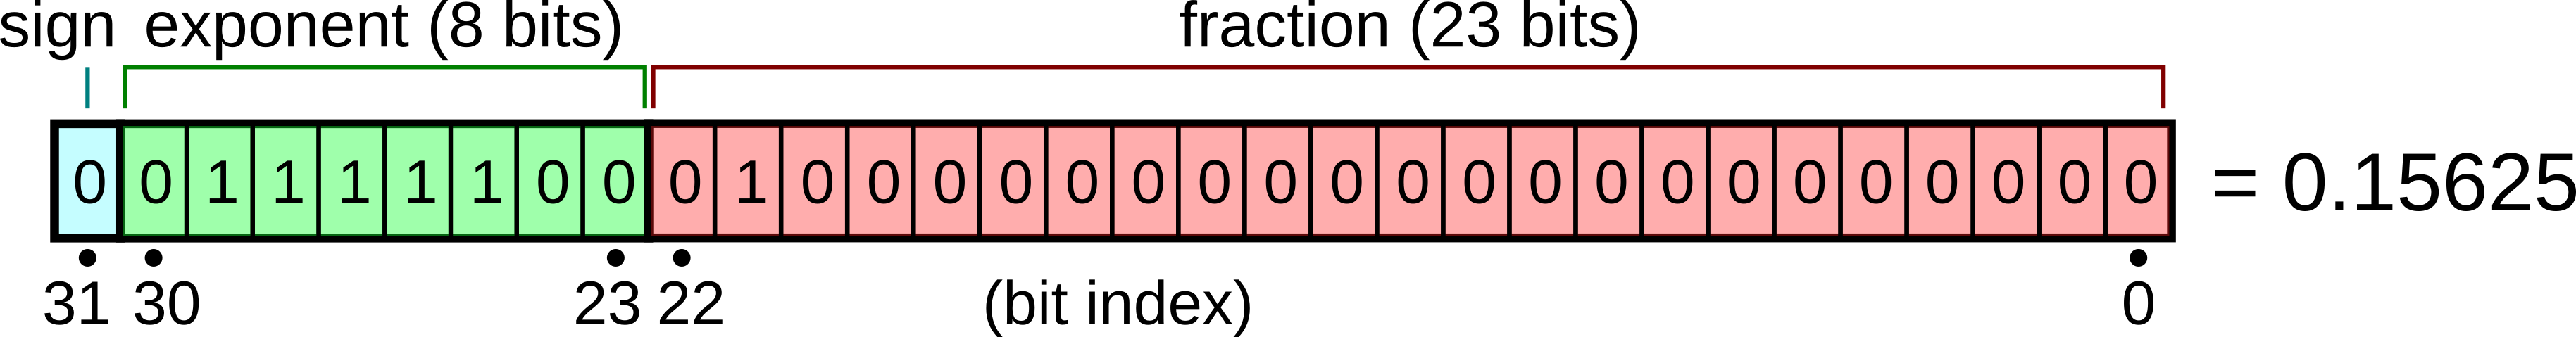
\includegraphics[width=\linewidth]{graphics/float.png}\label{obr:binary32}
32-bitový datový typ pro čísla s plovoucí řádovou tečkou je dle standardu uložen v konfiguraci $\langle s,e,f \rangle=\langle 1,8,23\rangle$.
\end{myfigure}
\end{example}

\subsection{Přesná reprezentace čísel jako hodnot}
Nyní se podívejme, jaká čísla uložená jako hodnoty považujeme za přesná. Projdeme opět všechny obory jako v první kapitole a poprvé propojíme matematickou teorii s informatickou realitou. Jako modelový jazyk nám poslouží C.

Všechny ukázky v této kapitole představují reálné chování představených datových typů na konkrétní AMD64 architektuře. Nejde teď tedy o žádnou teorii a jen ukazuji reálné limity. Na 128-bitové architektuře mohou být tyto limity jiné a typy použitelnější. Nicméně tato práce směřuje k přesným výpočtům rekurzivních čísel bez ohledu na architekturu.

\subsubsection{Přirozená čísla}
Přirozená čísla jsou uzavřena na operace sčítání a násobení. V počítači se jako hodnoty ukládají pomocí váženého pozičního kódu a tento má horní limit, jak velké číslo lze na dané architektuře uložit. Takto uložená přirozená čísla ovšem nejsou na operace uzavřena, protože může dojít k přetečení -- číslo ukládané se liší od čísla uloženého. Příklad tohoto chování vydíme na Obrázku \ref{obr:uinty}.
\begin{myfigure}{H}
\caption{Přirozená čísla v jazyce C}
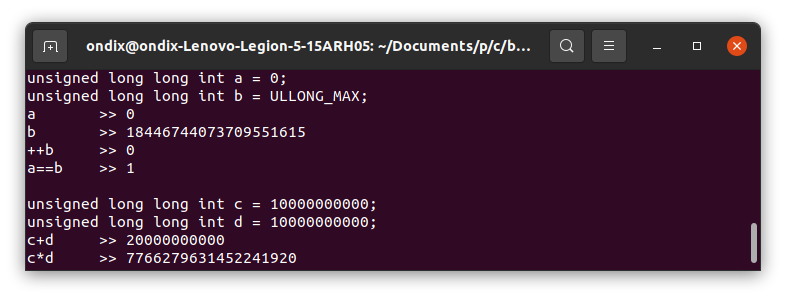
\includegraphics[width=\linewidth]{./graphics/uinty.png}\label{obr:uinty}
Největším datovým typem, který pracuje s přirozenými čísly je v jazyce C typ \texttt{unsigned long long int} a na 64-bitové architektuře umí uchovat čísla v intervalu $[0, 2^{64}-1]$. Na příkladu vidíme přetečení u inkrementace i násobení.
\end{myfigure}
Pokud ale ukládáme přirozené číslo v intervalu, ve kterém jej zvládne uložit datový typ jako hodnotu, můžeme ho považovat za přesné.

\subsubsection{Celá čísla}
Celá čísla jsou uzavřena na sčítání, odčítání a násobení. V paměti počítače se pak musí používat kódování záporných čísel jako hodnot, často jde o dvojkový komplement. Opět zde vyvstává problém s limity jakéhokoli hodnotového datového typu, totiž že vyjadřitelná čísla jsou ohraničená a hrozí přetečení (a i podtečení). Implementace celého čísla jako hodnoty tedy není na operace uzavřená (Obr. \ref{obr:inty}).
\begin{myfigure}{H}
\caption{Celá čísla v jazyce C}
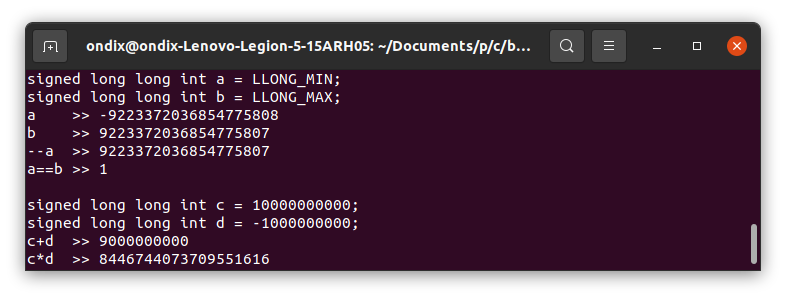
\includegraphics[width=\linewidth]{./graphics/inty.png}\label{obr:inty}
Nejširší datový typ jazyka C, který umí uložit celá čísla je \texttt{signed long long int}. Ten na 64-bitové architektuře zvládne uložit čísla z intervalu $[-2^{63}, 2^{63}-1]$. Na příkladu vidíme, že není uzavřen vůči operacím a že dochází k podtékání.
\end{myfigure}
Pakliže ukládáme celé číslo jako hodnotu, která se vejde do datového typu bez přetečení nebo podtečení, lze takto vyjádřené číslo považovat za přesné.

\subsubsection{Racionální čísla}
Racionální číslo se v jazyce C ukládá jako číslo s plovoucí řádovou tečkou. S~největší přesností se ukládá datový typ \texttt{long double}. Není specifikováno, jak má být přesný, pouze že má být minimálně tak přesný jako \texttt{double} \cite{wiki:LD}. Čísla, která jsou různá, ale kvůli zaokrouhlení se vyjádří jako stejná hodnota plovoucího čísla, jsou v~tomto směru potom nerozeznatelná. Každý plovoucí typ pak má garantovanou přesnost, na kterou by se různá čísla neměla reprezentovat stejně.

\begin{myfigure}{H}
\caption{Racionální čísla v jazyce C}
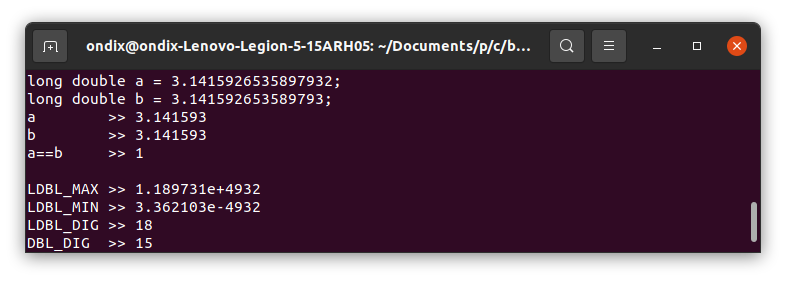
\includegraphics[width=\linewidth]{./graphics/floaty.png}\label{obr:floaty}
Nejrozsáhlejším datovým typem čísla s plovoucí řádovou tečkou je v jazyce C \texttt{long double}. Na příkladu vidíme, že jeho přesnost by měla být 18 desetinných míst, ale už na patnácti místech jsou dvě různá zapisovaná čísla zapsána stejně. Někde se tedy stala chyba a přesnost \texttt{long double} je stejná jako \texttt{double}, ale knihovna \texttt{float.h} to nereflektuje.
\end{myfigure}

Racionální čísla vyjádřená jako plovoucí můžeme považovat za přesná, pokud se nedostaneme mimo interval a přesnost stanovenou typem. Na Obrázku \ref{obr:floaty} vidíme, že rozsah datového typu \texttt{long double} je téměř $10^4$ řádů a přesnost je maximálně 15 desetinných míst. Čísla s plovoucí řádovou tečkou jsou nejlepší přiblížení k racionálním číslům, které lze vyjádřit jako hodnoty.

\subsection{Přesná reprezentace čísel jako struktur}
Již víme, že některá čísla lze přesně uložit jejich hodnotou. Nicméně standardní datové typy mají své limity, například přetékání nebo nedostatečná přesnost. Číslo je však namísto hodnotového datového typu reprezentovat typem referenčním. V kapitole \ref{kap:cisla} bylo nastíněno, že stejné číslo lze vyjádřit několika symboly, i když jeho hodnota je pouze jedna. Takto reprezentovaná čísla umíme velmi dobře v počítači vyjadřovat. Struktury v této podkapitole jsou pouze teoretickými koncepty bez konkrétní implementace.

\subsubsection{Přirozená čísla}
Jak bylo ukázáno v minulé podkapitole, přirozená čísla jsou uzavřena na sčítání a násobení, \texttt{unsigned int} ovšem nikoli. Cílem je tedy vymyslet strukturu, která dokáže reprezentovat jakékoli přirozené číslo. Jako hodnoty umíme na $n$ bytech uložit čísla $0$ až $2^n-1$, proto by pro přirozená čísla bylo možné adekvátně upravovat toto $n$.Velikost čísla by pak byla omezena jen velikostí paměti.

Struktura představující přirozené číslo musí zajišťovat, aby jeho hodnota při aplikaci matematických operací nepřetekla. Pokud struktura obdrží požadavek na násobení nebo sčítání, musí mít připravený další prostor a tam posunout bity, které by normálně přetekly. To je možné zajistit tak, že ve svém pomyslném paměťovém prostoru bude vždy po provedení operace procházet svých levých $2^{n-1}$ bitů, a pokud zde najde alespoň jednu jedničku, požádá o alokaci dalšího prostoru o velikost $2^n$, tedy zvedne $n$ o~jedna.

Pak už bude na operačním systému, kolik paměti bude moci struktuře přiřadit. Tato paměť je vždy prakticky omezená, teoreticky je však neomezená. Strukturu si tedy lze představit jako pouhý chytrý řadič bloků paměti za sebe. Pak lze \textit{naprosto přesně} zapsat jakékoli přirozené číslo. Paměťově toto není příliš efektivní, jedná se však o funkční princip. Optimalizace je ponechána až na konkrétní implementace.

\subsubsection{Celá čísla}
Situace v případě celých čísel je velmi podobná jako u přirozených čísel. Kromě přetečení navíc hrozí také podtečení, protože celá čísla musí být uzavřena i na odčítání. 

Vytvořme strukturu pro celé číslo jako dvojici přirozeného čísla a příznaku kladnosti. Metody struktury pak budou jen nastavovat příznak kladnosti -- u násobení jako exklusivní disjunkci, odčítání odpovídá sčítání s negací příznaku a u sčítání se příznak nastaví podle příznaku u většího čísla. Takto vytvořené struktury pak \textit{naprosto přesně} reprezentují jakékoli celé číslo.

\subsubsection{Racionální čísla}
Racionální čísla jsme definovali jako podíl celého a nenulového celého čísla. Racionální čísla (bez nuly) jsou uzavřená i na dělení. Zaveďme teď racionální číslo jako dvojici celých čísel (čitatele a jmenovatele) s invariantem, že druhé číslo nesmí být nikdy nula a že obě čísla jsou nesoudělná.

Násobení bude fungovat jako násobení na složkách, dělení pak bude jen prohození obou složek druhého argumentu a následné násobení. Odčítání je sčítání s opačným číslem a sčítání musí najít společný jmenovatel a poté specificky přenásobovat jednotlivé operandy.

Metody musí stále kontrolovat, zda nedochází k dělení nulou. Po konci výpočtu musí dojít ke zkrácení obou složek čísla. Predikát rovnosti dvou racionálních čísel kvůli podmínce nesoudělnosti je pak jednoduchý a je to rovnost na složkách.

Tato struktura je \textit{naprosto přesnou} reprezentací racionálních čísel. Jazyk Lisp implementuje racionální čísla zmíněným způsobem a nabízí datový typ \texttt{ratio}.

\subsection{Reálná čísla}
Předchozí číselné obory lze s dostatkem paměti naprosto přesně reprezentovat. Zbývají už jen iracionální čísla a máme všechna reálná čísla v přesné reprezentaci. Těch je nepočitatelně mnoho, a tak je není možné vytvořit z přirozených čísel nabalováním struktur jako předchozí obory. Nic jiného ale v paměti, která pracuje s diskrétními hodnotami, neumíme vytvořit.

Dosud jsme mluvili o \textit{naprosto přesných} číslech, struktura vyjadřující přesné číslo však může být i taková, která počítá jen přibližná čísla, nastavitelně vzdálená od (neznámé) přesné hodnoty. Takových čísel je počitatelně mnoho a říkáme jim čísla rekurzivní. Ve skutečnosti je právě hranice mezi racionálními čísly a rekurzivními čísly ta velká bariéra, která odděluje svět, kde vše funguje relativně jednoduše a ten, kde je všechno o řád těžší.

\subsubsection{Představa}\label{kap:predstava}
Než struktury definovat imperativně pomocí definic, jak by co měla implementovat, se spíše pokusím o definici struktury deklarativně, čili pomocí vlastností, které by měla splňovat.

Abstraktní struktura reprezentující reálné číslo by měla umožnit
\begin{itemize}
\item{jeho vyčíslení -- když struktura existuje, pak po zavolání vhodného nástroje je výsledkem hodnota, kterou tato struktura představuje;}
\item{přesnost -- i když má číslo nekonečný rozvoj nebo je velmi velké, abstrakce umožňuje jeho vyčíslení na danou přesnost v konečném čase;}
\item{podporovat matematické operace -- ve smyslu kapitoly \ref{operace_s_cisly};}
\item{podporovat matematické funkce -- ve smyslu kapitoly \ref{funkce_cisel};}
\item{být vracena jako výsledek funkce -- mít jasně popsanou strukturu, aby se dala rozšiřovat funkčnost;}
\item{být použita jako argument nějaké funkce -- typicky funkce pro vyčíslení.}
\end{itemize}

První dvě podmínky jsou přímo esenciální -- zajišťují, že abstrakce mohou reprezentovat reálná čísla na libovolnou (kladnou) přenost. Kdykoli budu potřebovat číslo dané konkrétní abstrakcí, zavolám příslušnou funkci s parametrem $\varepsilon$ reprezentujícím přesnost, na kterou toto číslo potřebuji. Obecně totiž nemusí být výsledkem vyčíslovací funkce přesná hodnota hledaného čísla, avšak díky těmto podmínkám budu výsledku vzdálen maximálně o zadanou hodnotu odchylky. \textit{Přesné} číslo tedy představuje číslo, které je od výsledku vzdálené o jasně definovanou hodnotu vyčíslitelné konečným výpočtem. Uvažujme strukturu $s_x$ přesně vyjadřující nějaké číslo $x$, zavolejme vyčíslovací funkci $enum$ a jako argumenty volme tuto strukturu a libovolné kladné $\varepsilon$, pak by výsledkem mělo být číslo $enum(s_x, \varepsilon)$ splňující nerovnost
\begin{equation}
|enum(s_x, \varepsilon)-x| \leq \varepsilon.
\end{equation}

Druhé dvě podmínky vštěpují dané struktuře reprezentující reálná čísla vlastnosti reálných čísel, a sice že s nimi jde sčítat, násobit atp. a že mohou být argumentem nějaké matematické funkce. Jistě nejde o to tyto struktury vkládat do stejných operací jako si představujeme s normálními čísly, například ve výrazu $3+4$ nechceme operandy nahrazovat abstraktními strukturami a očekávat správný výsledek, nýbrž chceme existenci ekvivalentní operace pro tyto struktury. To nutně neznamená, že musí být skutečně někde implementována, ale potřebujeme docílit stavu, kdy existence této není dokazatelně vyloučena.

Třetí a poslední dvě podmínky jsou spíše návod pro praktické použití těchto hypotetických struktur, aby se s nimi dalo smysluplně pracovat. To vlastně znamená, že musí být elementy prvního řádu (\textit{first-class citizen}), čili implementovány jako niterná součást použitého jazyka a ne jako svébytná konstrukce, která sice funguje, ale je nekompatibilní s jazykem svého vzniku, takže je vlastně nepoužitelná, uživatelsky nerozšiřitelná.

\subsubsection{Existující nástroje}\FloatBarrier
Nyní se podíváme, co na poli vyčíslování reálných čísel existuje v současné době.
\paragraph{Mpmath \cite{mpmath}}
\texttt{mpmath} je velmi rozsáhlá knihovna pro Python. Je publikována pod licensí BSD a je dosažitelná i pomocí \texttt{pip}u. Kromě základní funkčnosti pro výpočet funkcí a operací s čísly jsou implementovány i funkce pro výpočet funkcí intervalů, určitých integrálů, podpora tvorby grafů a mnoho dalšího. Dokumentace je velice hezky zpracovaná se spoustou příkladů. Přesnost se nastavuje proměnnou \texttt{mp.dps}. Jde o počet vypisovaných míst. Knihovna oplývá tolika možnostmi, že dokonce existuje stránka pro výpočet Ludolfova čísla sty možnými one-linery. Knihovna používá tři vlastní datové typy a sice \texttt{mpf} pro reálná čísla, \texttt{mpc} pro komplexní čísla a \texttt{matrix} pro matice. Příklad použití je na Obrázku \ref{obr:mpmath}.

\begin{myfigure}{}
\caption{Používání knihovny \texttt{mpmath}}
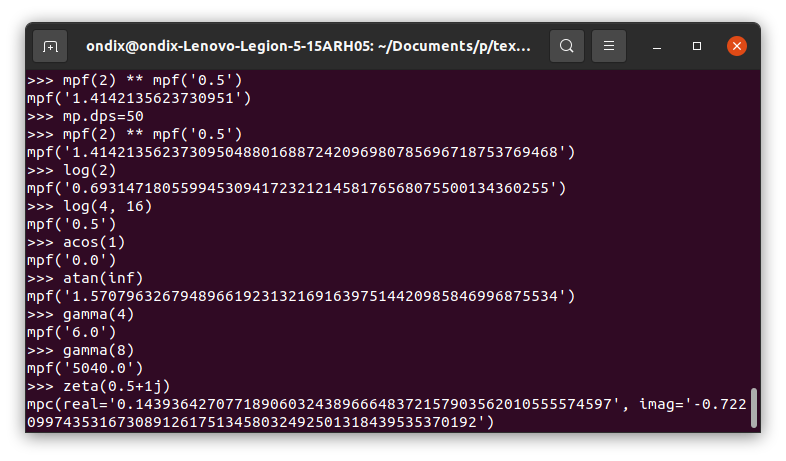
\includegraphics[width=\linewidth]{./graphics/mpmath.png}\label{obr:mpmath}
Struktura \texttt{mpf} podporuje matematické operace, na příkladu je vyobrazena odmocnina ze dvou. Ta je zde ve dvou provedeních, s defaultní přesností a s nastavenou na 50. Ukázány jsou i další matematické funkce, jmenovitě logaritmus, cyklometrické, gamma a Riemannovu zeta funkci, na jejímž vstupu i výstupu vidíme komplexní číslo.
\end{myfigure}

\paragraph{JScience \cite{jscience}}
\texttt{JScience} je knihovna pro jazyk Java. Její část pro práci s jednotkami se dostala do knihovny \texttt{javax}. Knihovna je široce rozkročena. Přináší podporu pro porovnávání a počítání jednotek z fyziky, geografie nebo ekonomie. Z matematiky je zde podpora pro jednoduchou symbolickou analýzu a strukturální algebru. Nás nejvíce zajímá část \texttt{org.jscience.mathematics.number}. Zde jsou zajímavé 3 datové typy a to \texttt{Real} umožnující základní výpočty s nastavitelnou přesností, \texttt{LargeInteger} ukládající velká celá čísla a \texttt{Rational} ukládající dvojice \texttt{LargeInteger}ů a umožňující jejich implicitní usměrňování a základní matematické operace. Příklad použití je na Obrázku \ref{obr:jscience}.

\begin{myfigure}{}
\caption{Používání knihovny \texttt{JScience}}
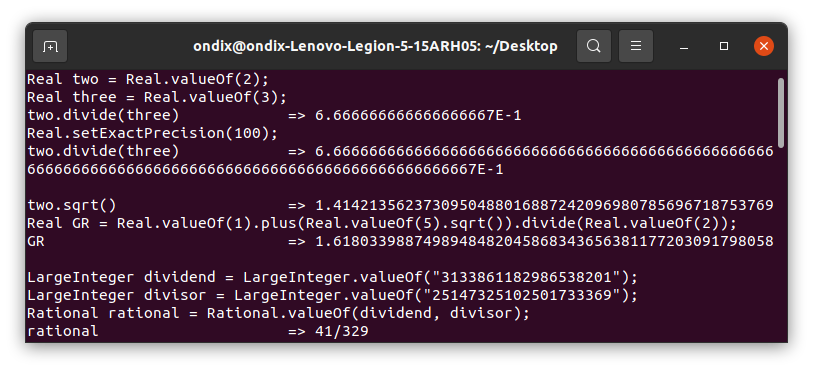
\includegraphics[width=\linewidth]{./graphics/jscience.png}\label{obr:jscience}
Na obrázku je ukázáno používání třídy \texttt{Real}. Operace jsou použitelné jako metody, nikoli operátorem. Konkrétně je představeno nastavování přesnosti, výpočet druhé odmocniny, zlatého řezu a zlomkové struktury s implicitním krácením.
\end{myfigure}

\paragraph{GNU Multiple Precision Arithmetic Library \cite{wiki:gmp} (GMP)}
\texttt{GMP} je knihovna pro jazyk C. Datový typ \texttt{mpz\_t} představuje celé číslo, u kterého nehrozí přetečení nebo podtečení. Zlomky velkých čísel představuje \texttt{mpq\_t} a operace podporují usměrňování. Přesný ekvivalent čísla s plovoucí řádovou tečkou představuje \texttt{mpf\_t}. Minimální počet bytů, ve kterém je uložen v paměti, se nastavuje funkcí \texttt{mpf\_set\_default\_prec}. Všechny typy implementují základní matematické operace. Protože je GMP součástí projektu GNU a protože je to knihovna pro C, je velmi mnoho nadstavbových knihoven, které její funkcionalitu využívají a rozšiřují. Z C-čkových jmenujme například \texttt{GNU MPFR}, která na je na GMP přímo založena \cite{wiki:mpfr} a přináší matematické funkce floatů, nebo \texttt{MPIR} -- paralelní projekt odtrhnuvší se od vývoje GMP a jdoucí svojí cestou, přesto snažící se implementovat rozhraní GMP, aby byly zastupitelné \cite{wiki:mpir}. Dále existují wrappery pro kompatibilitu s jinými jazyky a tudíž je GMP velmi rozšířená, ač se to nemusí uživateli zdát. Například pro platformu .NET je to knihovna \texttt{Math.GMP.Native}, pro Python \texttt{gmpy}, pro R \texttt{gmp}. Příklad použití je na Obrázku \ref{obr:gmp}.

\begin{myfigure}{}
\caption{Používání knihovny \texttt{GMP}}
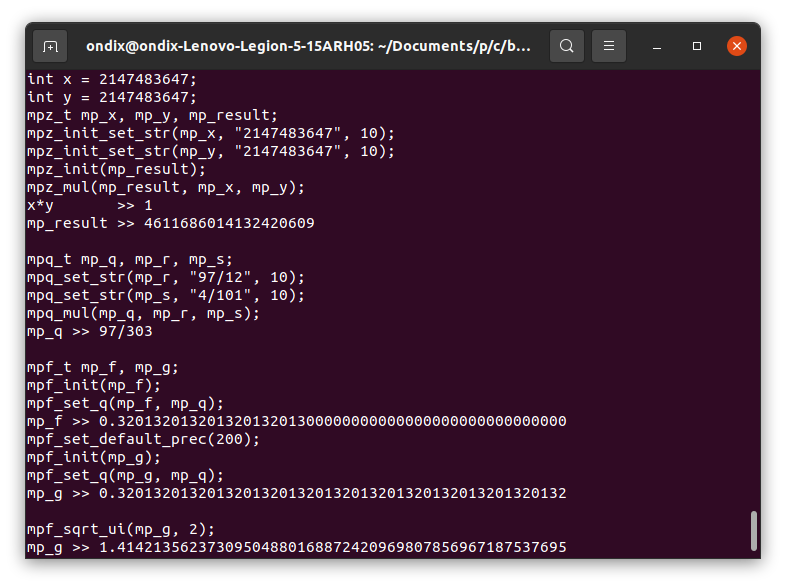
\includegraphics[width=\linewidth]{./graphics/gmp.png}\label{obr:gmp}
Na příkladu vidíme nejprve porovnání násobení klasických \texttt{int}ů versus struktur typu \texttt{mpz\_t}. U \texttt{int}ů dojde k přetečení, u mpz nikoli. Dále vidíme práci se zlomky, jejich inicializaci ze \texttt{string}u a násobení. Nakonec vidíme základní operace s typem \texttt{mpf\_t}, protějškem čísel s plovoucí řádovou tečkou.
\end{myfigure}

\paragraph{Class Library for Numbers \cite{wiki:CLN} (CLN)} \texttt{CLN} je knihovna pro jazyk C++ a je zdarma šířená pod licensí GPL. Implementuje čísla s~plovoucí řádovou tečkou racionální čísla jako zlomky, navíc komplexní čísla. Za přesná se považují racionální čísla a komplexní čísla s přesnou imaginární i reálnou částí. Plovoucí čísla pak typově přesně kopírují Lispovské a lze je tedy tedy použít k Lispovským implementacím. Zkratku CLN je tedy možné chápat i jako \uv{Common Lisp Numbers}. Nepřímé použití je na Obrázku \ref{obr:clisp}.
	
\begin{myfigure}{}
\caption{Implicitní používání knihovny \texttt{CLN}}
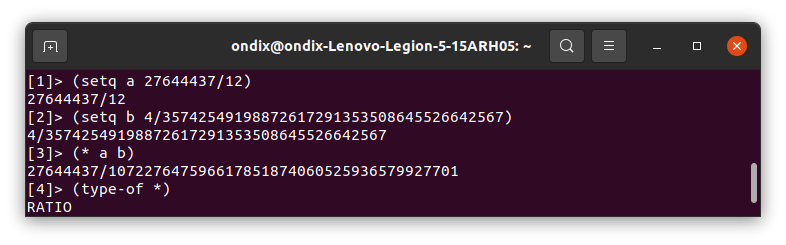
\includegraphics[width=\linewidth]{./graphics/clisp.png}\label{obr:clisp}
Knihovnu CLN používá CLisp, interpret jazyka Lisp. Využívá implementace čísel. Příklad ukazuje, že se zlomky automaticky zkracují. Že je CLisp založen na CLN usuzuji podle osoby Bruna Heible-a, který figuruje jako autor jak u CLN, tak u CLisp-u.
\end{myfigure}

\paragraph{Computable-reals \cite{gh:cr}}\label{kap:computable-reals}
\texttt{computable-reals} je Lispovská knihovna. Je volně ke stažení a dokonce k dostání pomocí \texttt{quicklisp}u. Podporuje základní funkcionalitu. Její funkce poznáme tak, že končí koncovkou \texttt{-r}. Vracené výsledky nejsou čísla, ale vlastního typu \texttt{C-REAL}. Defaultně se tisknou výsledky na 20 míst, ale nastavením proměnné \texttt{*print-prec*} se tento počet dá měnit \cite{lpb:numbers}. Kromě odmocniny jsou zde třeba základní násobky čísla $\pi$, logaritmy, mocniny, základní goniometrické funkce, arcus tangens. Knihovna se používá jako kalkulačka s nastavitelnou přesností. Příklad použití je na Obrázku \ref{obr:computable-reals}.

\begin{myfigure}{}
\caption{Používání knihovny \texttt{computable-reals}}
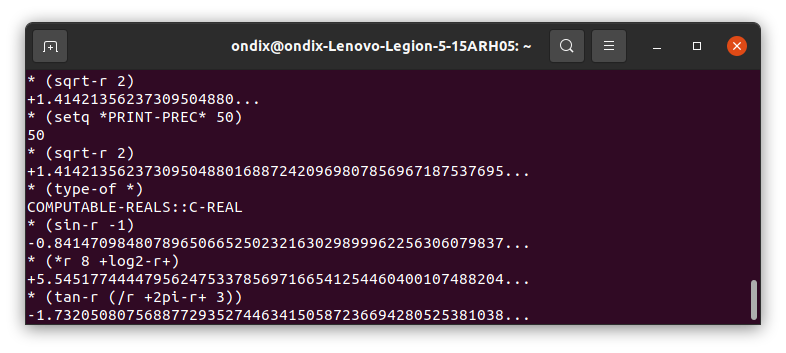
\includegraphics[width=\linewidth]{./graphics/computable-reals.png}\label{obr:computable-reals}
Na příkladu vidíme výpis odmocniny ze dvou na různé přesnosti, operace násobení a  několik matematických funkcí.
\end{myfigure}\FloatBarrier

\paragraph{Cíl práce}
Tolik tedy k strukturám již nyní implementujícím čísla a jejich operace, případně funkce. V některých implementacích se jedná o třídy, v jiných jde o strukturované datové typy. V následujícím textu se pokusíme navázat tam, kde končí naprostá přesnost nad racionálními čísly jazyka Lisp a naprogramujeme knihovnu přinášející některá iracionální čísla.

V této práci nám jde o přesnost a nikoli o rychlost a proto jako nativní typy budu používat právě zlomky, ačkoli pro rychlé operace s desetinnými čísly se používají plovoucí čísla, které mají často i hardwarovou podporu v jednotce FPU. Ostatně proto jsou v Lispu i plovoucí typy \cite{PS:PCL}.

K programování jsem jako textový editor použil \textit{Visual Studio Code} s rozšířením \textit{Rainbow Brackets} a jako překladač \textit{SBCL}.
\mypart{Implementace}
V implementační části propojíme teoreticky orientované výsledky s aplikovaným aspektem a dáme vzniknout knihovně \texttt{tnums}. Jak jsem napsal výše, všechna čísla i manipulaci s nimi lze vyjádřit jako funkce. Nejpřímější aplikace tohoto poznání tedy vede k užití funkcionálního paradigmatu. Jako jeho zástupce byl vedoucím práce zvolen Lisp. Nejprve se podíváme na jednoduché převody mezi reprezentacemi v Lispu a tnumy, poté se podíváme na matematické operace tnumů a nakonec také na matematické funkce tnumů.
\section{Tnumy}
Struktury jsou dány jako funkce jedné proměnné -- přesnosti. Je potřeba je matematicky nadefinovat a poté v Lispu vymodelovat.

\subsection{Vztah čísel a tnumů}
Funkce, kterými budu modelovat rekurzivní čísla a které budu poté v Lispu implementovat nazývám \textit{True Numbers}, zkráceně \textit{tnums}. Jsou totiž opravdovější než čísla, která jsou uložena jako hodnoty, čímž ztrácí na přesnosti. Vzniknuvší knihovna se pak jmenuje \texttt{tnums}.

\begin{definition}[Tnum]\label{def:tnum}
Funkce $\tnum{x}:(0,1)\rightarrow\mathbb{Q}$, která pro všechna $\varepsilon\in (0,1)$ vrací hodnotu $\txe$ splňující nerovnost
\begin{equation}\label{rov:def:tnum}
|\txe - x |\leq \varepsilon
\end{equation}
se nazývá \textit{tnum} \normalfont{[ti:n{\textturnv}m]} čísla $x$.

Množinu všech tnumů čísla $x$ značíme $\Tnum{x},(\forall x \in\mathbb{R})(\Tnum{x}=\{\tnum{x}|(\forall\varepsilon\in (0,1)):|\txe-x|\leq\varepsilon\})$. Množinu všech tnumů pak značíme symbolem $\mathfrak{T}$.
\end{definition}

Tnum $\tnum{x}$ je struktura představující rekurzivní číslo $x$. Při výpočtu jeho hodnoty nejprve tento tnum vytvoříme (výpočetně rychlé), a pak ho necháme vyčíslit, tj. zavolat s přesností (výpočetně pomalé). Vyčíslení tedy odkládáme na nejpozdější možnou dobu, mluvíme o líném vyhodnocování.

Tnumy přesných čísel lze vyčíslit s dokonalou přesností. Lisp přesně reprezentuje všechna racionální čísla. To je ve shodě s principem vyčíslení rekurzivního čísla. Pomocí $\tnum{r}(\varepsilon)$ tedy získáváme $q$ z nerovnice \eqref{rov:rac_u_real} a též $enum(s_r,\varepsilon)$ z nerovnice \eqref{ner:struktura}. Číslo, jak ho chápe Lisp dále označuji \textit{num}.

\begin{lemma}[O numu jako tnumu]\label{lem:num-to-tnum}
Pro všechna $x\in\mathbb{R}$ a všechna $\varepsilon \in (0,1)$ platí: číslo $\txe$ lze nahradit číslem $x$.
\begin{proof}
Z nerovnosti \eqref{rov:def:tnum} získáváme $|\txe - x |\leq \varepsilon$. Po dosazení $\txe := x$ pak $|x - x | = 0 \leq \varepsilon$, což platí pro všechna $x\in\mathbb{R}$ i $\varepsilon\in{(0,1)}$.
\end{proof}
\end{lemma}

Nejpřesnější reprezentace čísla je toto číslo samotné. Lisp pracuje i se zlomky (datový typ \texttt{ratio}), proto mohou být přesná všechna racionální čísla.

\begin{lispcode}{\texttt{num-to-tnum}}{Funkce převádějící num na tnum}
(\textcolor{funkcionalni}{defun} \textcolor{pojmenovan}{num-to-tnum} (num)
  (\textcolor{vedlejsi}{let} ((rat_num (\textcolor{matematicke}{rationalize} num)))
    (\textcolor{funkcionalni}{lambda} (eps) (\textcolor{vedlejsi}{declare} (\textcolor{vedlejsi}{ignore} eps))
      rat_num)))
\end{lispcode}

Převod opačným směrem je přímočarý. Chceme-li číslo $x\in\mathbb{R}$ s~přesností $\varepsilon\in{(0,1)}$, stačí zavolat $\txe$. Mimo přípustný interval $\varepsilon$ chápeme jako $10^{-|\varepsilon|}$.

\begin{lemma}[O převodu tnumu na num]
Pokud existuje funkce $\tnum{x}\in\Tnum{x}$, pak po zavolání s argumentem $\varepsilon$ vrací hodnotu $\txe$ splňující $(|\txe - x |\leq \varepsilon)$.
\begin{proof}
Plyne přímo z definice \ref{def:tnum}.
\end{proof}
\end{lemma}

\begin{lispcode}{\texttt{rat-expt}}{Funkce pro racionální umocňování}
(\textcolor{funkcionalni}{defun} \textcolor{pojmenovan}{rat-expt} (num exp)
  (\textcolor{matematicke}{rationalize} (\textcolor{matematicke}{expt} num exp)))
\end{lispcode}

\begin{lispcode}{\texttt{tnum-to-num}}{Funkce převádějící tnum na num}
(\textcolor{funkcionalni}{defun} \textcolor{pojmenovan}{tnum-to-num} (tnum eps)
  (\textcolor{funkcionalni}{when} (\textcolor{funkcionalni}{or} (\textcolor{matematicke}{>=} 0 eps) (\textcolor{matematicke}{<=} 1 eps))
    (\textcolor{vedlejsi}{setf} eps (\textcolor{moje}{rat-expt} 10 (\textcolor{matematicke}{-} (\textcolor{matematicke}{abs} eps)))))
  (\textcolor{funkcionalni}{funcall} tnum (\textcolor{matematicke}{rationalize} eps)))
\end{lispcode}

Z čísla na tnum je převod jednoduchý, opačným směrem lze převádět jen, pokud tnum existuje. V knihovně teď jsou jen tnumy racionálních čísel a aparát pro převody mezi $\mathfrak{T}$ a $\mathbb{Q}$. Teď půjde o tvorbu co nejvíce tnumů iracionálních čísel.

\subsection{Ludolfovo číslo}
První iracionální konstantou, která do knihovny přibude je Ludolfovo číslo.

\begin{definition}[Ludolfovo číslo \cite{piratio}]
Ludolfovo číslo $\pi$ je dáno jako poměr obvodu kružnice k jejímu průměru.
\end{definition}

Ludolfovo číslo je nejslavnější transcendentní konstanta, pro jejíž vyčíslení existuje přemnoho vzorců, například vzorec Leibnizův: $\pi=4\sum_{n\in\mathbb{N}}\frac{(-1)^n}{2n+1}$ \cite{approxpi}.

Rychleji konverguje řada v BBP (tvůrci Bailey, Borwein, Plouffe) vzorci.

\begin{fact}[Kohoutkový BBP vzorec \cite{BBP}]
\begin{equation}\label{rov:pi-rada}
\pi=\sum_{i\in\mathbb{N}}\frac{1}{16^i}\left(\frac{4}{8i+1}-\frac{2}{8i+4}-\frac{1}{8i+5}-\frac{1}{8i+6}\right).
\end{equation}
\end{fact}

Máme řadu čísla, jež chceme přidat do \texttt{tnums}. Výraz v závorce je pro $i>0$\\ menší než jedna. Proto lze každý $i$-tý člen, kde $i>0$, zhora omezit $16^{-i}$. Omezující členy tvoří geometrickou řadu, jejíž zbytek je dle faktu \ref{vet:o_zbytku_geometricke_rady} roven $\frac{1}{16^i*15}$. Platí\\
\begin{equation}
\left|\pi - \sum_{i=0}^n\frac{1}{16^i}\left(\frac{4}{8i+1}-\frac{2}{8i+4}-\frac{1}{8i+5}-\frac{1}{8i+6}\right) \right| \leq \frac{1}{16^n*15}.
\end{equation}

\begin{consequence}[Tnum Ludolfova čísla]
Nechť $\tnum{}()$ je funkce s předpisem 
\begin{equation}
\tnum{}()(\varepsilon)=\left[\begin{array}{l}
\mathrm{1.~}\text{Najdi~nějaké~}n\in\mathbb{N}^+\text{~tak,~aby~}/(16^n15)\leq\varepsilon;\\
\mathrm{2.~}\text{Vrať~}\sum_{i=0}^n\frac{1}{16^i}\left(\frac{4}{8i+1}-\frac{2}{8i+4}-\frac{1}{8i+5}-\frac{1}{8i+6}\right),
\end{array}\right.
\end{equation} pak $\tnum{}\in\Tnum{\pi}$.
\end{consequence}
\begin{lispcode}{\texttt{tnum-pi}}{Funkce pro tnum Ludolfova čísla}
(\textcolor{funkcionalni}{defun} \textcolor{pojmenovan}{tnum-pi} ()
  (\textcolor{funkcionalni}{lambda} (eps)
    (\textcolor{vedlejsi}{let} ((result 0))
      (\textcolor{funkcionalni}{loop} \textcolor{obarvi}{for} i \textcolor{obarvi}{from} 0
            \textcolor{obarvi}{for} /16powi = (\textcolor{matematicke}{expt} 16 (\textcolor{matematicke}{-} i)) \textcolor{obarvi}{and} 8i = (\textcolor{matematicke}{*} 8 i)
            \textcolor{obarvi}{do} (\textcolor{vedlejsi}{incf} result 
                     (\textcolor{matematicke}{*} /16powi
                        (\textcolor{matematicke}{-} (\textcolor{matematicke}{/} 4 (\textcolor{matematicke}{+} 8i 1))
                           (\textcolor{matematicke}{/} 2 (\textcolor{matematicke}{+} 8i 4))
                           (\textcolor{matematicke}{/} (\textcolor{matematicke}{+} 8i 5))
                           (\textcolor{matematicke}{/} (\textcolor{matematicke}{+} 8i 6)))))
            \textcolor{obarvi}{until} (\textcolor{matematicke}{<=} (\textcolor{matematicke}{/} /16powi 15) eps)
            \textcolor{obarvi}{finally} (\textcolor{funkcionalni}{return} result)))))
\end{lispcode}

\subsection{Přenásobování numem}

Racionální násobky tnumů umožní vyčíslení například čísla $2\pi{/3}$.

\begin{theorem}[O přenásobení tnumu racionální konstantou]
Nechť $c\in\mathbb{Q}$, $\tnum{x}\in\Tnum{x},x\in\mathbb{R}$ a funkce $\tnum{}(\tnum{x},c)$ má předpis
\begin{equation}
\tnum{}(\tnum{x},c)(\varepsilon)=\begin{cases}c*\tnum{x}\left(\frac{\varepsilon}{|c|}\right) & \text{pro~}c\neq{0},\\0&\text{pro~}c={0},\end{cases}
\end{equation}
pak $\tnum{}(\tnum{x},c)\in\Tnum{x*c}$.
\begin{proof}
Pokud přenásobíme jakékoli číslo nulou, je výsledkem nula (agresivní prvek vůči násobení). Znění věty pro nenulovou konstantu dokážeme tak, že z předpokladu $|\txe -x|\leq\varepsilon$ odvodíme $|c*\tnum{x}(\frac{\varepsilon}{|c|})-c*x|\leq\varepsilon$. Protože pracujeme s nerovnicemi, budeme postupovat dvěmi větvemi -- pro $c$ kladné a záporné.

Z definice tnumu předpokládáme
\begin{equation}
|\txe-x|\leq\varepsilon,
\end{equation}
po přenásobení kladným $c>0$ dostáváme
\begin{equation}
c*|\txe-x|\leq c*\varepsilon,
\end{equation}
protože je ale $c$ kladné, lze jím absolutní hodnotu roznásobit
\begin{equation}
|c*\txe-c*x|\leq c*\varepsilon,
\end{equation}
a nyní na pravé straně potřebujeme dostat přesnost $\varepsilon$. Protože dle definice platí $|\tnum{y}(\varepsilon)-y|\leq\varepsilon$, platí jistě i $|\tnum{y}(\frac{\varepsilon}{c})-y|\leq\frac{\varepsilon}{c}$, pak ale musí platit i
\begin{equation}
\left|c*\tnum{x}\left(\frac{\varepsilon}{c}\right)-c*x\right|\leq \varepsilon.
\end{equation}
Pro zápornou konstantu je důkaz podobný, a protože jako argument tnumů bereme kladné číslo, přibývá v děliteli v argumentu tnumu ještě absolutní hodnota. Dohromady pak získáváme
\begin{equation}
\left|c*\tnum{x}\left(\frac{\varepsilon}{|c|}\right)-c*x\right|\leq\varepsilon,
\end{equation}
což jsme chtěli odvodit.
\end{proof}
\end{theorem}

\begin{lispcode}{\texttt{tnum*num}}{Funkce přenásobující tnum racionální konstantou}
(\textcolor{funkcionalni}{defun} \textcolor{pojmenovan}{tnum*num} (tnum num)
  (\textcolor{vedlejsi}{let} ((rat_num (\textcolor{matematicke}{rationalize} num)))
    (\textcolor{funkcionalni}{lambda} (eps)
      (\textcolor{funkcionalni}{if} (\textcolor{funkcionalni}{zerop} num)
          (\textcolor{moje}{num-to-tnum} 0)
        (\textcolor{matematicke}{*} (\textcolor{moje}{tnum-to-num} tnum (\textcolor{matematicke}{/} eps (\textcolor{matematicke}{abs} rat_num))) rat_num))))) 
\end{lispcode}

\begin{consequence}[Opačný tnum]\label{dusl:negace_tnumu}
Nechť $\tnum{x}\in\Tnum{x}, x\in\mathbb{R}$ a funkce $\tnum{}(\tnum{x})$ má předpis
\begin{equation}
\tnum{}(\tnum{x})(\varepsilon)=-\txe,
\end{equation}
pak $\tnum{}(\tnum{x})\in\Tnum{-x}$.
\begin{proof}
Protože $-x = (-1)x$ a $|-1|=1$, pak z přechozí věty dostáváme $-\txe=(-1)\txe=(-1)\tnum{x}(\frac{\varepsilon}{1})=(-1)\tnum{x}(\frac{\varepsilon}{|-1|})=\tnum{(-1)x}(\varepsilon)=\tnum{-x}(\varepsilon)\in\Tnum{-x}$.
\end{proof}
\end{consequence}

\begin{lispcode}{\texttt{-tnum}}{Funkce pro opačný tnum}
(\textcolor{funkcionalni}{defun} \textcolor{pojmenovan}{-tnum} (tnum)
  (\textcolor{funkcionalni}{lambda} (eps)
    (\textcolor{matematicke}{-} (\textcolor{moje}{tnum-to-num} tnum eps))))
\end{lispcode}


\clearpage
\section{Operace tnumů}
Implementace matematických operací je různě složitá. Zatímco aditivní operace jsou celkem jednoduché, multiplikativní jsou řádově složitější, tak mocninné dokončíme až na konci následující kapitoly.

\subsection{Aditivní operace}
Operace \texttt{+} bere přirozený počet argumentů. Pro žádný vrací nulu (neutrální prvek aditivní grupy \cite{RachALG1}), pro jeden vrací tento a pro více pak jejich součet (je třeba doprogramovat součet). Operace \texttt{-} potom vyžaduje alespoň jeden argument, v případě zadání pouze tohoto se vrací tnum k němu opačný, v případě více pak jejich rozdíl (je třeba doprogramovat rozdíl).

\begin{theorem}[O součtu tnumů]
Nechť $\tnum{x_0}\in\Tnum{x_0}, \tnum{x_1}\in\Tnum{x_1}, \ldots, \tnum{x_n}\in\Tnum{x_n}$ a funkce $\tnum{}(\tnum{x_0},\tnum{x_1},\ldots,\tnum{x_n})$ má předpis
\begin{equation}
\tnum{}(\tnum{x_0},\tnum{x_1},\ldots,\tnum{x_n})(\varepsilon)=\sum_{i=0}^n\tnum{x_i}\left(\frac{\varepsilon}{n+1}\right),
\end{equation}
pak $\tnum{}(\tnum{x_0},\tnum{x_1},\ldots,\tnum{x_n})\in\Tnum{x_0+x_1+\ldots{+}x_n}$.

\begin{proof}
Předpokládejme $\tnum{x_i}(\varepsilon) + \varepsilon \geq x_i$ a $\tnum{x_i}(\varepsilon) - \varepsilon \leq x_i$ pro $i \in \{0, 1, \ldots , n\}$ a ukažme $\sum_{i=0}^n\tnum{x_i}\left(\frac{\varepsilon}{n+1}\right) + \varepsilon \geq \sum_{i=0}^nx_i$ a $\sum_{i=0}^n\tnum{x_i}\left(\frac{\varepsilon}{n+1}\right) - \varepsilon \leq \sum_{i=0}^nx_i$.

Z definice tnumu předpokládáme
\begin{equation}
\begin{aligned}
\tnum{x_0}\left(\frac{\varepsilon}{n+1}\right)+\frac{\varepsilon}{n+1}\geq x_0 &\land \tnum{x_0}\left(\frac{\varepsilon}{n+1}\right)-\frac{\varepsilon}{n+1}\leq x_0,\\
&\ldots \\
\tnum{x_n}\left(\frac{\varepsilon}{n+1}\right)+\frac{\varepsilon}{n+1}\geq x_n &\land \tnum{x_n}\left(\frac{\varepsilon}{n+1}\right)-\frac{\varepsilon}{n+1}\leq x_n.\\
\end{aligned}
\end{equation}
Sečtěme teď všechny výrazy a získáváme
\begin{equation}
\sum_{i=0}^n\tnum{x_i}\left(\frac{\varepsilon}{n+1}\right) + \sum_{i=0}^n\frac{\varepsilon}{n+1} \geq \sum_{i=0}^nx_i \land \sum_{i=0}^n\tnum{x_i}\left(\frac{\varepsilon}{n+1}\right) - \sum_{i=0}^n\frac{\varepsilon}{n+1} \leq \sum_{i=0}^nx_i,
\end{equation}
dále $\sum_{i=0}^n\frac{\varepsilon}{n+1} = \varepsilon$, takže
\begin{equation}
\sum_{i=0}^n\tnum{x_i}\left(\frac{\varepsilon}{n+1}\right) + \varepsilon \geq \sum_{i=0}^nx_i \land \sum_{i=0}^n\tnum{x_i}\left(\frac{\varepsilon}{n+1}\right) - \varepsilon \leq \sum_{i=0}^nx_i,
\end{equation}
což jsme chtěli ukázat.
\end{proof}
\end{theorem}

\begin{lispcode}{\texttt{tnum+}}{Funkce na součet tnumů}
(\textcolor{funkcionalni}{defun} \textcolor{pojmenovan}{tnum+} (&rest tnums)
  (\textcolor{funkcionalni}{if} (\textcolor{funkcionalni}{null} tnums)
      (\textcolor{moje}{num-to-tnum} 0)
    (\textcolor{funkcionalni}{lambda} (eps)
      (\textcolor{vedlejsi}{let} ((new-eps (\textcolor{matematicke}{/} eps (\textcolor{funkcionalni}{list-length} tnums))))
        (\textcolor{funkcionalni}{apply} \textquotesingle\textcolor{moje}{+} 
               (\textcolor{funkcionalni}{mapcar} (\textcolor{funkcionalni}{lambda} (tnum) 
                         (\textcolor{moje}{tnum-to-num} tnum new-eps))
                       tnums))))))
\end{lispcode}

\begin{fact}[Rozdíl tnumů]
Nechť $\tnum{x_{i}}\in\Tnum{x_{i}}, x\in\mathbb{R}$ pro $i\in\{-1,0,\ldots,n\}$ a funkce $\tnum{}(\tnum{x_{-1}},\tnum{x_0},\ldots,\tnum{x_n})$ má předpis
\begin{equation}
\tnum{}(\tnum{x_{-1}},\tnum{x_0},\ldots,\tnum{x_n})(\varepsilon)=\tnum{x_{-1}-\sum_{i=0}^nx_n}(\varepsilon)=\tnum{x_{-1}+\left(-\sum_{i=0}^nx_n\right)}(\varepsilon),
\end{equation}
pak $\tnum{}(\tnum{x_{-1}},\tnum{x_0},\ldots,\tnum{x_n})\in\Tnum{x_{-1}-x_0-\ldots -x_n}$.
\end{fact}

\begin{lispcode}{\texttt{tnum-}}{Funkce pro opačný tnum a rozdíl tnumů}
(\textcolor{funkcionalni}{defun} \textcolor{pojmenovan}{tnum-} (tnum1 &rest tnums)
  (\textcolor{funkcionalni}{if} (\textcolor{funkcionalni}{null} tnums)
      (\textcolor{moje}{-tnum} tnum1)
    (\textcolor{moje}{tnum+} tnum1 (\textcolor{moje}{-tnum} (\textcolor{funkcionalni}{apply} \textquotesingle\textcolor{moje}{tnum+} tnums)))))
\end{lispcode}

\subsection{Multiplikativní operace}
Jako první multiplikativní operaci představím převrácení hodnoty tnumu. Je to unární operace jako Opačný tnum, jen jde o jinou inverzi. Protože převrácení pracuje jen s nenulovými čísly, přidáme ještě aparát pro tnumy nenulových čísel.

\begin{definition}[Nenulový tnum]
Tnum $\tnum{}$, který nikdy nenabývá nulové hodnoty, neboli $(\forall \varepsilon \in (0,1))(\tnum{}(\varepsilon) \neq 0)$ budeme nazývat \textit{nenulový tnum} a budeme jej značit $\tnum{}_\emptyset$.
\end{definition}

Nenulová čísla tedy budeme moci reprezentovat nenulovými tnumy.

\begin{definition}[Bezpečné epsilon]\label{def:bezpecne_epsilon}
K libovolnému $\varepsilon\in (0,1)$ a tnumu $\tnum{x}\in\Tnum{x}, x\neq 0$ uvažujeme číslo $\varepsilon_\emptyset(\tnum{x},\varepsilon)$ tak, že
\begin{enumerate}
\item{$0<\varepsilon_\emptyset(\tnum{x},\varepsilon)\leq\varepsilon$},
\item{$\tnum{x}(\varepsilon_\emptyset(\tnum{x},\varepsilon)) \neq 0$} a
\item{$|\tnum{x}(\varepsilon_\emptyset(\tnum{x},\varepsilon))| > \varepsilon_\emptyset(\tnum{x},\varepsilon)$}
\end{enumerate}
a nazýváme jej \textit{bezpečným epsilonem}.
\end{definition}

\begin{lemma}[O nenulovém tnumu nenulového čísla]\label{vet:nenul}
Tnum nenulového čísla lze vyčíslit nenulově, čili $(\forall x \in(\mathbb{R}\setminus\{0\}))((\exists \tnum{x}) \rightarrow (\exists \tnum{x}_\emptyset))$. 
\begin{proof}
Vezměme za $\tnum{x}_\emptyset$ funkci $\tnum{}$, s předpisem $\tnum{}(\varepsilon) = \tnum{x}(\varepsilon_\emptyset(\tnum{x},\varepsilon))$. Pak díky podmínce $1$ v definici \ref{def:bezpecne_epsilon} vyčíslení proběhne v pořádku a díky bodu $2$ ve stejné definici bude vyčíslení nenulové, díky čemuž se jedná o nenulový tnum.
\end{proof}
\end{lemma}

Bezpečných epsilonů je nekonečně mnoho, stačí nám najít jediné. Funkce pro jeho výpočet potřebuje tnum a epsilon. To je ve shodě se zavedeným symbolem $\varepsilon_\emptyset(\tnum{x}, \varepsilon)$. Dále musí kvůli kontrole nenulovosti vypočítat i num zadaného tnumu a musí také vracet nové epsilon. Aby se tnum nevyčísloval vícekrát, když už jeho hodnotu známe, vrací funkce i tento num.

\begin{lispcode}{\texttt{get-nonzero-num+eps}}{Funkce pro nalezení bezpečného epsilonu a numu nenulového tnumu}
(\textcolor{funkcionalni}{defun} \textcolor{pojmenovan}{get-nonzero-num+eps} (tnum eps)
  (\textcolor{vedlejsi}{let} ((num (\textcolor{moje}{tnum-to-num} tnum eps)))
    (\textcolor{funkcionalni}{if} (\textcolor{funkcionalni}{or} (\textcolor{funkcionalni}{zerop} num) (\textcolor{matematicke}{<=} (\textcolor{matematicke}{abs} num) eps))
        (\textcolor{moje}{get-nonzero-num+eps} tnum (\textcolor{matematicke}{/} eps 10))
      (\textcolor{matematicke}{values} num eps))))
\end{lispcode}

\begin{theorem}[O převráceném tnumu]\label{hyp:prevraceni_tnumu}
Nechť $\tnum{x}\in\Tnum{x},x\neq 0$ a funkce $\tnum{}(\tnum{x})$ má předpis
\begin{equation}
\tnum{}(\tnum{x})(\varepsilon)=/\left[\tnum{x}(\varepsilon_\emptyset(\tnum{x}, (\varepsilon*|\tnum{x}(\varepsilon_\emptyset(\tnum{x}, \varepsilon))|*(|\tnum{x}(\varepsilon_\emptyset(\tnum{x}, \varepsilon))|-\varepsilon_\emptyset(\tnum{x}, \varepsilon)))))\right],
\end{equation}
pak $\tnum{}(\tnum{x})\in\Tnum{/x}$.
\begin{proof}

Podle rovnice \eqref{rov:def:tnum} platí 
\begin{equation}
\left|\txe-x\right|\leq \varepsilon,
\end{equation}
což lze díky lemmatu \ref{vet:nenul} a předpokladu nenulovosti $x$ přepsat na
\begin{equation}
\left|\tnum{x}(\varepsilon_\emptyset(\tnum{x}, \varepsilon))-x\right|\leq \varepsilon,
\end{equation}
díky absolutní hodnotě pak platí
\begin{equation}
\left| x-\tnum{x}(\varepsilon_\emptyset(\tnum{x}, \varepsilon))\right|\leq \varepsilon.
\end{equation}
Nerovnici vydělíme kladným číslem $|\tnum{x}(\varepsilon_\emptyset(\tnum{x}, \varepsilon))*x|$
\begin{equation}
\frac{\left| x-\tnum{x}(\varepsilon_\emptyset(\tnum{x}, \varepsilon))\right|}{|\tnum{x}(\varepsilon_\emptyset(\tnum{x}, \varepsilon))*x|}\leq \frac{\varepsilon}{|\tnum{x}(\varepsilon_\emptyset(\tnum{x}, \varepsilon))*x|}
\end{equation}
a protože $|a|*|b|=|a*b|$, po dvojí aplikaci platí
\begin{equation}
\left|\frac{x-\tnum{x}(\varepsilon_\emptyset(\tnum{x}, \varepsilon))}{\tnum{x}(\varepsilon_\emptyset(\tnum{x}, \varepsilon))*x}\right|\leq \frac{\varepsilon}{|\tnum{x}(\varepsilon_\emptyset(\tnum{x}, \varepsilon))|*|x|}
\end{equation}
a po roztržení levého výrazu na rozdílné jmenovatele dostáváme
\begin{equation}
\left|\frac{1}{\tnum{x}(\varepsilon_\emptyset(\tnum{x}, \varepsilon))}-\frac{1}{x}\right|\leq \frac{\varepsilon}{|\tnum{x}(\varepsilon_\emptyset(\tnum{x}, \varepsilon))|*|x|}.
\end{equation}
Dále díky předpokladu $3$ z definice \ref{def:bezpecne_epsilon} $|x|\geq|\tnum{x}(\varepsilon_\emptyset(\tnum{x}, \varepsilon))|-\varepsilon_\emptyset(\tnum{x}, \varepsilon)$ a proto
\begin{equation}
\left|\frac{1}{\tnum{x}(\varepsilon_\emptyset(\tnum{x}, \varepsilon))}-\frac{1}{x}\right|\leq \frac{\varepsilon}{|\tnum{x}(\varepsilon_\emptyset(\tnum{x}, \varepsilon))|*(|\tnum{x}(\varepsilon_\emptyset(\tnum{x}, \varepsilon))|-\varepsilon_\emptyset(\tnum{x}, \varepsilon))},
\end{equation}
takže po úpravě přesnosti dostáváme
\begin{equation}
\left|\frac{1}{\tnum{x}(\varepsilon_\emptyset(\tnum{x}, (\varepsilon * |\tnum{x}(\varepsilon_\emptyset(\tnum{x}, \varepsilon))|*(|\tnum{x}(\varepsilon_\emptyset(\tnum{x}, \varepsilon))|-\varepsilon_\emptyset(\tnum{x}, \varepsilon)))))}-\frac{1}{x}\right|\leq \varepsilon.
\end{equation}
\end{proof}
\end{theorem}

\begin{lispcode}{\texttt{/tnum}}{Funkce pro převracenou hodnotu tnumu}
(\textcolor{funkcionalni}{defun} \textcolor{pojmenovan}{/tnum} (tnum)
  (\textcolor{funkcionalni}{lambda} (eps)
    (\textcolor{matematicke}{multiple-value-bind} (num eps0)
        (\textcolor{moje}{get-nonzero-num+eps} tnum eps)
      (\textcolor{vedlejsi}{let*} ((absnum (\textcolor{matematicke}{abs} num))
             (neweps (\textcolor{matematicke}{*} eps absnum (\textcolor{matematicke}{-} absnum eps0))))
        (\textcolor{matematicke}{/} (\textcolor{funkcionalni}{if} (\textcolor{matematicke}{>=} neweps eps) num
             (\textcolor{moje}{get-nonzero-num+eps} tnum neweps)))))))
\end{lispcode}

Operace \texttt{*} bere přirozený počet argumentů. Pro žádný vrací jedničku (neutrální prvek multiplikativní grupy \cite{RachALG1}), pro jeden vrací tento a pro více pak jejich součin (doprogramovat zbývá součin).

\begin{theorem}[O součinu dvou tnumů]\label{vet:soucin_dvou_tnumu}
Nechť $\tnum{x}\in\Tnum{x},x\in\mathbb{R}$ a $\tnum{y}\in\Tnum{y},y\in\mathbb{R}$ a funkce $\tnum{}(\tnum{x},\tnum{y})$ má předpis
\begin{equation}
\tnum{}(\tnum{x},\tnum{y})(\varepsilon)=\tnum{x}\left(\frac{\varepsilon}{2*\mathrm{max}\left\{(|\tnum{y}(\varepsilon)| + \varepsilon);1\right\}}\right)*\tnum{y}\left(\frac{\varepsilon}{2*\mathrm{max}\left\{(|\tnum{x}(\varepsilon)| + \varepsilon);1\right\}}\right),
\end{equation}
pak $\tnum{}(\tnum{x},\tnum{y})\in\Tnum{x*y}$.

\begin{proof}
\begin{itemize}\item{
Nejprve si dokažme nerovnici
\begin{equation}\label{ner:abst}
|x|\leq|\tnum{x}(\varepsilon)|+\varepsilon.
\end{equation}
Odečtením $|\tnum{x}(\varepsilon)|$ získáváme
\begin{equation}
|x|-|\tnum{x}(\varepsilon)|\leq\varepsilon,
\end{equation}
což bude platit, pokud dokážeme silnější tvrzení
\begin{equation}
||x|-|\tnum{x}(\varepsilon)||\leq\varepsilon.
\end{equation}
To díky trojúhelníkové nerovnosti $||a|-|b||\leq|a-b|$ lze přepsat na
\begin{equation}
|x-\tnum{x}(\varepsilon)|\leq\varepsilon,
\end{equation}
v absolutní hodnotě můžeme prohodit sčítance beze změny její hodnoty. Získaný vztah
\begin{equation}
|\tnum{x}(\varepsilon)-x|\leq\varepsilon
\end{equation}
platí přímo z definice tnumu.}

\item{Nerovnice
\begin{equation}\label{ner:abst2}
\frac{|y|}{\mathrm{max}\left\{(|\tnum{y}(\varepsilon)| + \varepsilon);1\right\}}\leq 1
\end{equation}
vyplývá z nerovnice \eqref{ner:abst}, ekvivalentně je ji totiž možné zapsat $\frac{|x|}{|\tnum{x}(\varepsilon)|+\varepsilon}\leq 1$ a maximum ve jmenovateli jen tvrzení posiluje.}

\item{Nerovnice
\begin{equation}\label{ner:abst3}
\frac{\left|\tnum{x}\left(\frac{\varepsilon}{2*\mathrm{max}\left\{(|\tnum{y}(\varepsilon)| + \varepsilon);1\right\}}\right)\right|}{\mathrm{max}\left\{(|\tnum{x}(\varepsilon)| + \varepsilon);1\right\}}\leq 1
\end{equation}
vyplývá ze skutečnosti, že $0\leq\frac{\varepsilon}{2*\mathrm{max}\{(|\tnum{y}(\varepsilon)+\varepsilon);1\}}\leq\varepsilon$ a proto
\begin{equation}
\frac{\left|\tnum{x}\left(\frac{\varepsilon}{2*\mathrm{max}\left\{(|\tnum{y}(\varepsilon)| + \varepsilon);1\right\}}\right)\right|}{\mathrm{max}\left\{(|\tnum{x}(\varepsilon)| + \varepsilon);1\right\}}\leq\frac{|\tnum{x}(\varepsilon)|+\varepsilon}{\mathrm{max}\left\{(|\tnum{x}(\varepsilon)| + \varepsilon);1\right\}}\leq 1,
\end{equation}což platí.}

\item{Nyní přejděme k důkazu věty. Aby věta platila, musí být splněna nerovnost
\begin{equation}
\left| \tnum{x}\left(\frac{\varepsilon}{2*\mathrm{max}\left\{(|\tnum{y}(\varepsilon)| + \varepsilon);1\right\}}\right)*\tnum{y}\left(\frac{\varepsilon}{2*\mathrm{max}\left\{(|\tnum{x}(\varepsilon)| + \varepsilon);1\right\}}\right) -xy \right|\leq\varepsilon.
\end{equation} V dalším kvůli přehlednosti zápisu budu označovat $\varepsilon_x := \frac{\varepsilon}{2*\mathrm{max}\left\{(|\tnum{y}(\varepsilon)| + \varepsilon);1\right\}}$ a $\varepsilon_y := \frac{\varepsilon}{2*\mathrm{max}\left\{(|\tnum{x}(\varepsilon)| + \varepsilon);1\right\}}$.

Rozepíšeme levou stranu, odečtením a přičtením členu $\tnum{x}(\varepsilon_x)*y$ dostáváme
\begin{equation}
|\tnum{x}(\varepsilon_x)*\tnum{y}(\varepsilon_y) - \tnum{x}(\varepsilon_x)*y + \tnum{x}(\varepsilon_x)*y - x*y|\leq
\end{equation}
a z trojúhelníkové nerovnosti
\begin{equation}
\leq|\tnum{x}(\varepsilon_x)*\tnum{y}(\varepsilon_y) - \tnum{x}(\varepsilon_x)y |+| \tnum{x}(\varepsilon_x)*y - x*y|\leq
\end{equation}
a po vytknutí $|\tnum{x}(\varepsilon_x)|$ z prvních dvou členů a $|y|$ z druhých dvou máme
\begin{equation}
\leq|\tnum{x}(\varepsilon_x)|*|\tnum{y}(\varepsilon_y) - y|+|y|*|\tnum{x}(\varepsilon_x) - x|\leq
\end{equation}
a po dvojím použití vztahu $|\tnum{x}(\varepsilon)-x|\leq\varepsilon$ získáváme
\begin{equation}
\begin{aligned}
\leq\frac{\varepsilon}{2}*|\tnum{x}(\varepsilon_x)|*\left|\frac{1}{\mathrm{max}\left\{(|\tnum{x}(\varepsilon)| + \varepsilon);1\right\}}\right|&+\\+\frac{\varepsilon}{2}*|y|*\left|\frac{1}{\mathrm{max}\left\{(|\tnum{y}(\varepsilon)| + \varepsilon);1\right\}}\right|&=
\end{aligned}
\end{equation}
a zjednodušíme-li zápis pomocí zlomku, dostáváme
\begin{equation}
= \frac{\varepsilon}{2}*\frac{\left|\tnum{x}(\varepsilon_x)\right|}{\mathrm{max}\left\{(|\tnum{x}(\varepsilon)| + \varepsilon);1\right\}}+\frac{\varepsilon}{2}*\frac{|y|}{\mathrm{max}\left\{(|\tnum{y}(\varepsilon)| + \varepsilon);1\right\}}\leq
\end{equation}
a díky dokázaným nerovnostem \eqref{ner:abst2} a \eqref{ner:abst3} pak platí
\begin{equation}
\leq\frac{\varepsilon}{2}+\frac{\varepsilon}{2}=\varepsilon.
\end{equation}}
\end{itemize}
\end{proof}
\end{theorem}

Právě dokázaná věta mluví o součinu dvou tnumů. Zobecnění na konečný počet tnumů by v tomto bodě šlo naprogramovat akumulací. To je ale neefektivní řešení a proto by bylo dobré najít obecnou funkci. Následující vztah není dokázaný, vychází však z tvaru násobení pro dva tnumy.

\begin{hypothesis}[Součin tnumů]\label{vet:soucin_tnumu}
Nechť $\tnum{x_i}\in\Tnum{x_i}, x_i\in\mathbb{R}$ pro $i=0,1,\ldots,n$ a funkce $\tnum{}(\tnum{x_0},\tnum{x_1},\ldots,\tnum{x_n})$ má předpis
\begin{equation}
\tnum{}(\tnum{x_0},\tnum{x_1},\ldots,\tnum{x_n})(\varepsilon)=\prod_{i=0}^n\tnum{x_i}\left(\frac{\varepsilon}{(n+1)*\mathrm{max}\left\{\prod_{j=0, i\neq j}^n(|\tnum{x_j}(\varepsilon)|+\varepsilon);1\right\}}\right),
\end{equation}
pak $\tnum{}(\tnum{x_0},\tnum{x_1},\ldots,\tnum{x_n})\in\Tnum{\prod_{i=0}^nx_i}$.
\end{hypothesis}

Věta mluví o nenulových číslech. Nesnižujeme ale obecnost, protože nula je agresivní prvek a výsledkem násobení čehokoli s nulou je nula, takže se ostatní numy ani nemusejí počítat a výsledek se může vrátit.

Samotná implementace pak využívá pomocnou mapovací funkci.

\begin{lispcode}{\texttt{create-list-for-multiplication}}{Pomocná fun\-kce pro násobení}
(\textcolor{funkcionalni}{defun} \textcolor{pojmenovan}{create-list-for-multiplication} (tnums eps)
  (\textcolor{vedlejsi}{let*} ((result nil) (len (\textcolor{funkcionalni}{list-length} tnums)) (el (\textcolor{matematicke}{/} eps len))
         (nums (\textcolor{funkcionalni}{mapcar} (\textcolor{funkcionalni}{lambda} (tnum) 
                         (\textcolor{moje}{tnum-to-num} tnum el)) tnums)))
    (\textcolor{funkcionalni}{dotimes} (i len result)
      (\textcolor{vedlejsi}{let} ((neps 1))
        (\textcolor{funkcionalni}{dotimes} (j len)
          (\textcolor{funkcionalni}{unless} (\textcolor{matematicke}{=} i j)
            (\textcolor{vedlejsi}{setf} neps (\textcolor{matematicke}{/} neps (\textcolor{matematicke}{+} (\textcolor{matematicke}{abs} (\textcolor{funkcionalni}{nth} j nums)) eps)))))
        (\textcolor{vedlejsi}{setf} result (cons
                      (\textcolor{funkcionalni}{if} (\textcolor{matematicke}{<=} neps 1) (\textcolor{funkcionalni}{nth} i nums)
                        (\textcolor{moje}{tnum-to-num} (\textcolor{funkcionalni}{nth} i tnums)
                                     (\textcolor{matematicke}{/} el (max neps 1))))
                      result))))))
\end{lispcode}

\begin{lispcode}{\texttt{tnum*}}{Funkce pro násobení tnumů}
(\textcolor{funkcionalni}{defun} \textcolor{pojmenovan}{tnum*} (&rest tnums)
  (\textcolor{funkcionalni}{if} (\textcolor{funkcionalni}{null} tnums)
      (\textcolor{moje}{num-to-tnum} 1)
    (\textcolor{funkcionalni}{lambda} (eps)
      (\textcolor{funkcionalni}{apply} \textquotesingle\textcolor{moje}{*} (\textcolor{moje}{create-list-for-multiplication} tnums eps)))))
\end{lispcode}

Operace \texttt{/} vyžaduje alespoň jeden argument, v případě zadání pouze tohoto vrací převrácený tnum, v případě více pak jejich podíl (zbývá doprogramovat podíl).

\begin{fact}[Podíl tnumů]
Nechť $\tnum{x_i}\in\Tnum{x_i},x_i\in\mathbb{R}\setminus\{0\}$ pro $i\in\{0,1,\ldots ,n\}$ a $x_{i}\in\mathbb{R}$ pro $i=-1$ a funkce $\tnum{}(\tnum{x_{-1}},\tnum{x_0},\ldots,\tnum{x_n})$ má předpis
\begin{equation}
\tnum{}(\tnum{x_{-1}},\tnum{x_0},\ldots,\tnum{x_n})=\tnum{x_{-1}/\prod_{i=0}^nx_i}=\tnum{x_{-1}*\left(/\prod_{i=0}^nx_i\right)},
\end{equation}
pak $\tnum{}(\tnum{x_{-1}},\tnum{x_0},\ldots,\tnum{x_n})\in\Tnum{x_{-1}/x_0/\ldots /x_n}$.
\end{fact}

\begin{lispcode}{\texttt{tnum/}}{Funkce pro dělení tnumů}
(\textcolor{funkcionalni}{defun} \textcolor{pojmenovan}{tnum/} (tnum1 &rest tnums)
  (\textcolor{funkcionalni}{if} (\textcolor{funkcionalni}{null} tnums)
      (\textcolor{moje}{/tnum} tnum1)
    (\textcolor{moje}{tnum*} tnum1 (\textcolor{moje}{/tnum} (\textcolor{funkcionalni}{apply} \textquotesingle\textcolor{moje}{tnum*} tnums)))))
\end{lispcode}

Pro tnumy $a, b\in\mathfrak{T}$ existuje tnum $a+b$ a $a*b$. Množina $\mathfrak{T}$ je tedy uzavřena na operace $\texttt{+}$ a $\texttt{*}$. Tnumy pak i z pohledu strukturální algebry dobře reprezentují rekurzivní čísla, ta jsou totiž číselným tělesem \cite{rice:kompr}.

\subsection{Mocninné operace}
K implementaci mocninných operací potřebujeme funkce, které přidáme až v další kapitole. Uveďme zde alespoň vztahy, podle kterých lze mocninné operace naprogramovat.

Obecná mocnina využívá přirozený logaritmus a exponenciálu
\begin{equation}\label{rov:obmoc}
a^b=e^{\mathrm{ln}(a)^b}=e^{(b*\mathrm{ln}(a))}.
\end{equation}

Odmocninu lze vyjádřit pomocí převrácení hodnoty mocniny
\begin{equation}\label{rov:odmoc}
\sqrt[b]{a}=a^{(/b)}.
\end{equation}
\clearpage
\section{Funkce tnumů}
Knihovna \texttt{tnums} v této chvíli umí přidávat racionální čísla, Ludolfovo číslo a provádět mezi nimi multiplikativní a aditivní operace. Bylo by vhodné teď přidat další rekurzivní čísla. Jejich dobrým zdrojem, jak jsem napsal již v~podkapitole \ref{funkce_cisel}, jsou matematické funkce. V této kapitole se podíváme na funkci exponenciální, šest funkcí goniometrických a přirozený logaritmus. Na konci potom dodělám matematické operace a tím bude knihovna v použitelné verzi hotová.

\subsection{Aproximace funkcí}
Představa funkce tnumu je, že bude opět vracet tnum. Chci totiž opět libovolnou přesnost a také umožnit zřetězování funkcí. Hledám pak formu aproximace, která bude umožňovat libovolně škálovat, jak blízko ke kýženému číslu se výpočet ukončí. Dobrým nástrojem k tomu jsou Taylorovy polynomy. Ty se snaží hledat hodnotu $T(x)$ tak, aby byla co nejblíže hledané hodnotě $f(x)$ tak, že z~nějakého bodu, kterému budeme říkat počátek, se co nejlépe snaží nepodobit průběh funkce, kterou aproximují. Pro funkci $f$ budu Taylorův polynom stupně $n$ se středem v $a$ značit $T^{f,a}_n$. Pro práci s Taylorovými polynomy potřebujeme ještě naprogramovat faktoriál přirozeného čísla. To bývá typická úloha na rekurzi -- té se ale vyhýbáme, protože pro velké vstupy může přetékat zásobník. Iterativní verze by tímto neduhem neměla trpět.

\begin{lispcode}{\texttt{factorial}}{Funkce pro výpočet faktoriálu přirozeného čísla}
(\textcolor{funkcionalni}{defun} \textcolor{pojmenovan}{factorial} (n)
  (\textcolor{vedlejsi}{let} ((result 1))
    (\textcolor{funkcionalni}{loop} \textcolor{obarvi}{for} i \textcolor{obarvi}{from} n \textcolor{obarvi}{downto} 1
      \textcolor{obarvi}{do} (\textcolor{vedlejsi}{setf} result (\textcolor{matematicke}{*} result i)))
    result))
\end{lispcode}

Podívejme se teď na to, jak se prakticky dá počítat aproximace funkce v bodě $x$. Nejjednodušší je vzít funkci $T^{f,a}_0(x) = f(a)$. Je to jednoduchá aproximace, která na velmi blízkém okolí bodu $a$ může fungovat i velmi uspokojivě. Lepší nápadem je vzít přímku, která se bude dotýkat grafu funkce $f$ v bodě $a$. Předpis takovéto bude $T^{f,a}_1(x) = f(a)+f'(a)(x-a)$. To už je lepší aproximace, protože nebere v úvahu jen hodnotu funkce $f$ v bodě $a$ ale i její první derivaci, takže víme více o směru, kam se možná bude pohybovat. Ještě lepším nápadem pak je vzít parabolu přimknutou k grafu funkce $f$ jako $T^{f,a}_2(x) = f(a)+f'(a)(x-a)+\frac{f''(a)}{2}(x-a)^2$. Teď už zohledňujeme funkční hodnotu, směr křivky i konvexnost. Ještě lepším nápadem je použít $T^{f,a}_3(x):y=f(a)+f'(a)(x-a)+\frac{f''(a)}{2}(x-a)^2+\frac{f'''(a)}{6}(x-a)^3\ldots$\cite{MTTP}.

\begin{remind}[Taylorova a Maclaurinova řada]
Kdybychom takto postupovali donekonečna (v limitním smyslu), dostali bychom Taylorovu řadu z definice \ref{def:taymac_rada}. Pro $a=0$ pak Taylorovu řadu nazýváme řadou Maclaurinovou.
\end{remind}

Lze odvodit, že pokud Taylorovy zbytky konvergují k nule, lze Taylorovou řadou $T_\infty^{f,a}$ nahradit funkci $f$ \cite{ZDVNNR}. Nám ale nestačí pouhá konvergence zbytků, ale chtěli bychom jejich velikost nějak omezovat. Nejprve si zkusme nějakou formou zbytky vyjádřit.

\begin{fact}[Taylorova věta \cite{TMA:Calculus}]
Nechť $f$ má spojité derivace až do řádu $n+1$ na nějakém intervalu obsahujícím $a$. Pak pro každé $x$ z tohoto intervalu máme Taylorův vzorec
\begin{equation}
f(x) = T_n^{f,a}(x) + R_n^{f,a}(x)\text{, kde}
\end{equation}
\begin{equation}\label{TP}
T_n^{f,a}(x) = \sum_{i=0}^{n}\frac{f{(i)}(a)}{i!}(x-a)^i,
\end{equation}
\begin{equation}\label{integralnitvar}
R_n^{f,a}(x)=\int_a^x\frac{(x-t)^n}{n!}f^{(n+1)}(t)dt.
\end{equation}
Navíc existuje číslo $\xi$, z intervalu s krajními body $x$ a $a$ takové, že
\begin{equation}\label{lagrangeuvtvar}
R_n^{f,a}(x)=\frac{f^{(n+1)}(\xi)}{(n+1)!}(x-a)^{n+1}.
\end{equation}
Pro důkaz vizte kapitolu 7.5 v \cite{TMA:Calculus}.
\end{fact}

Součet v rovnici \ref{TP} nazýváme Taylorův polynom funkce $f$ stupně $n$ v bodě $a$, $R_n^{f,a}(x)$ nazýváme $n$-tým Taylorovým zbytkem. Vyjádření \ref{integralnitvar} pak říkáme \textit{integrální tvar} zbytku a \ref{lagrangeuvtvar} je Lagrangeův tvar zbytku \cite{MTTP}.

Když už máme vyjádřeny zbytky, můžeme se pokusit je zhora omezovat, stejně jako tomu bylo u geometrické řady. Ve skutečnosti nám na celou kapitolu vystačí pouze tyto dva mechanismy, tedy \textit{Taylorův zbytek} a \textit{Zbytek geometrické řady}.

\subsection{Exponenciála}
Exponenciála je funkce s předpisem $\mathrm{exp}(x) = e^x$ kde $e$ je tzv. \textit{Eulerovo číslo} definované $e=\lim_{n\to\infty}\left(1+\frac{1}{n}\right)^n$ \cite{EPJVMAI}. To je transcendentní konstanta a je to též základ přirozeného logaritmu. Exponenciále se proto také dá říkat přirozená mocnina. Ještě podotkněme, že $\frac{d}{dx}\mathrm{exp}(x)=\mathrm{exp}(x)$.

\begin{myremark}{Značení exponenciály}
Mimo informatickou oblast jsem si nikde nevšiml, že by se exponenciála čísla $x$ značila jinak než $e^x$, mé značení $\mathrm{exp}(x)$ tedy možná působí neadekvátně. V dalším textu ale používám i pouze funkci ($\mathrm{exp}$), nikoli její hodnotu ($\mathrm{exp}(x)$) a zápis $e^x$ umožňuje jen toto druhé použití. Proto se omlouvám matematickému čtenáři za neintuitivní značení, ale je zde důvodné. Navíc lépe vyjadřuje, že je exponenciála funkcí.
\end{myremark}

\subsubsection{Exponenciála čísla}

\begin{fact}[Exponenciála jako Maclaurinova řada \cite{ZDVNNR}]\label{vet:exp_jako_rada}
Funkci $\mathrm{exp}(x)$ lze vyjádřit jako Maclaurinovu řadu ve tvaru
\begin{equation}
\mathrm{exp}(x) = \underset{i \in \mathbb{N}}{\sum} \frac{x^i}{i!} = \frac{1}{1} + \frac{x}{1} + \frac{x^2}{2!} + \frac{x^3}{3!} + \ldots
\end{equation}
Pro důkaz vizte podkapitolu \ref{duk:exp_jako_rada} v příloze \ref{pril:dukazy}.
\end{fact}

Podívejme se nyní na zbytek této řady. Když rozepíšeme Lagrangeův tvar, získáváme pro nějaké $\xi\in(0,x)$
\begin{equation}
R_n^{exp, 0}(x) = \frac{e^\xi}{(n+1)!}x^{n+1}.
\end{equation}

Podotkněme, že exponenciála je rostoucí a že $e<2.72$ a proto
\begin{equation}
(\forall\xi\in (0,x))(\mathrm{exp}(\xi)<\mathrm{exp}(x) < 2.72^x).
\end{equation}

Když vše poskládáme dohromady, získáváme aproximaci exponenciály na shora omezenou přesnost, pro $x\in\mathbb{R}$ platí
\begin{fact}[Omezení Taylorova zbytku exponenciály]
\begin{equation}
|R_n^{exp, 0}(x)| = \left|\mathrm{exp}(x)- \sum_{i=0}^n \frac{x^i}{i!}\right| \leq \left| \frac{2.72^x}{(n+1)!}x^{n+1} \right|.
\end{equation}
\end{fact}

\begin{consequence}[O tnumu exponenciály numu]
Pro všechna $\varepsilon$ existuje $n\in\mathbb{N}^+$ tak, aby $\left|\frac{2.72^x}{(n+1)!}x^{n+1}\right| \leq \varepsilon$ a pak
\begin{equation}
\mathcal{T}^{\mathrm{exp}(x)}(\varepsilon)=\sum_{i=0}^n \frac{x^i}{i!}.
\end{equation}
\begin{proof}
Existence čísla $n$ je zřejmá z definice limity posloupnosti a z toho, že limita podílu polynomu a faktoriálu je rovna nule.

Dále protože $\mathrm{exp}(x) = T^{exp, 0}_n(x)+R^{exp, 0}_n(x)$, lze psát
\begin{equation}
T^{exp, 0}_n(x) \in [\mathrm{exp}(x) - |R^{exp, 0}_n(x)|, \mathrm{exp}(x) + |R^{exp, 0}_n(x)|],
\end{equation}
přičemž dle předchozího faktu platí
\begin{equation}
T^{exp, 0}_n(x) \in [\mathrm{exp}(x) - \left| \frac{2.72^x}{(n+1)!}x^{n+1} \right|, \mathrm{exp}(x) + \left| \frac{2.72^x}{(n+1)!}x^{n+1} \right|]
\end{equation}
a z předpokladu pak
\begin{equation}
T^{exp, 0}_n(x) \in [\mathrm{exp}(x) - \varepsilon, \mathrm{exp}(x) + \varepsilon]
\end{equation}
a tedy
\begin{equation}\label{eq:tat}
\mathcal{T}^{\mathrm{exp}(x)}(\varepsilon) = T^{exp, 0}_n(x).
\end{equation}
\end{proof}
\end{consequence}

Při implementaci stačí jen iterovat přes $n$, dokud nebude právě odvozené omezení zbytku menší než kýžená přesnost. Stejný přístup jsme viděli již u Ludolfova čísla.

\begin{lispcode}{\texttt{num-exp}}{Funkce pro výpočet exponenciály čísla na danou přesnost}
(\textcolor{funkcionalni}{defun} \textcolor{pojmenovan}{num-exp} (num eps)
  (\textcolor{vedlejsi}{let} ((above (\textcolor{moje}{rat-expt} 272/100 num)) (n 0)
      (nfact 1) (xpown 1) (result 1))
    (\textcolor{funkcionalni}{loop} 
      \textcolor{obarvi}{until} (\textcolor{matematicke}{<=} (\textcolor{matematicke}{/} (\textcolor{matematicke}{*} above xpown) nfact) eps)
      \textcolor{obarvi}{do} (progn
        (\textcolor{vedlejsi}{incf} n)
        (\textcolor{vedlejsi}{setf} nfact (\textcolor{moje}{factorial} n)
          xpown (\textcolor{matematicke}{expt} num n))
        (\textcolor{vedlejsi}{incf} result (\textcolor{matematicke}{/} xpown nfact)))
      \textcolor{obarvi}{finally} (\textcolor{funkcionalni}{return} result))))
\end{lispcode}

\begin{myremarkbez}{Eulerovo číslo jako exponenciála}
Protože triviálně platí $e = e^1$, můžu do knihovny přidat i samotné Eulerovo číslo jako jednoduchou uživatelskou funkci.
\begin{lispcode}{\texttt{tnum-e}}{Funkce pro $\mathcal{T}^e$\hfill$\blacksquare$}
(\textcolor{funkcionalni}{defun} \textcolor{pojmenovan}{tnum-e} ()
  (\textcolor{funkcionalni}{lambda} (eps)
    (\textcolor{moje}{num-exp} 1 eps)))
\end{lispcode}
\end{myremarkbez}

Už tedy umíme exponenciálu čísla na danou přesnost. Teď jsme tedy ve stádiu, kdy lze pro $q\in\mathbb{Q}$ napsat
\begin{equation}
\mathcal{T}^{\mathrm{exp}(q)}=\texttt{(num-exp } q \texttt{)}.
\end{equation}
To není malý výsledek, bohužel nás ale sotva uspokojí. Nyní ještě musíme rozšířit funkcionalitu na všechna reálná čísla, která mají tnum. Opět jde o linku rozdílu mezi racionálními a rekurzivními čísly, která prochází celou prací.

\subsubsection{Exponenciála tnumu}
Víme, že $\mathcal{T}^x(\varepsilon) \in [x-\varepsilon,x+\varepsilon]$, podívejme se, jak se chová přesnost čísla po projití exponenciální funkcí.

\begin{myfigure}{H}
\caption{Obraz přesnosti po průchodu exponenciálou}
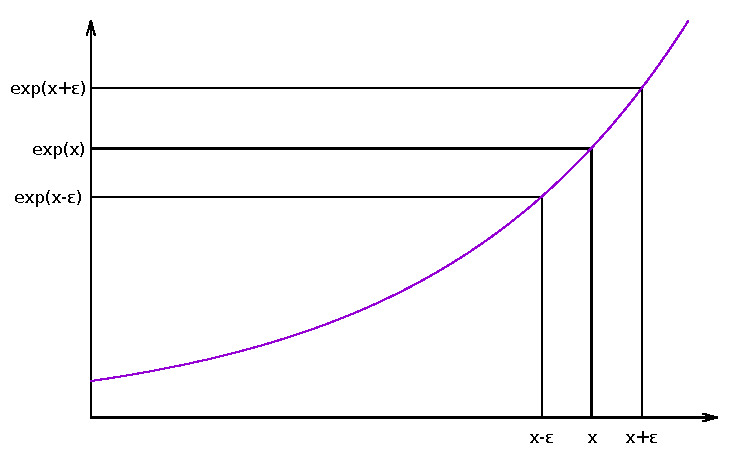
\includegraphics[width=\linewidth]{graphics/exp1.pdf}\label{fig:exp1}
Horní interval je vyšší než spodní.

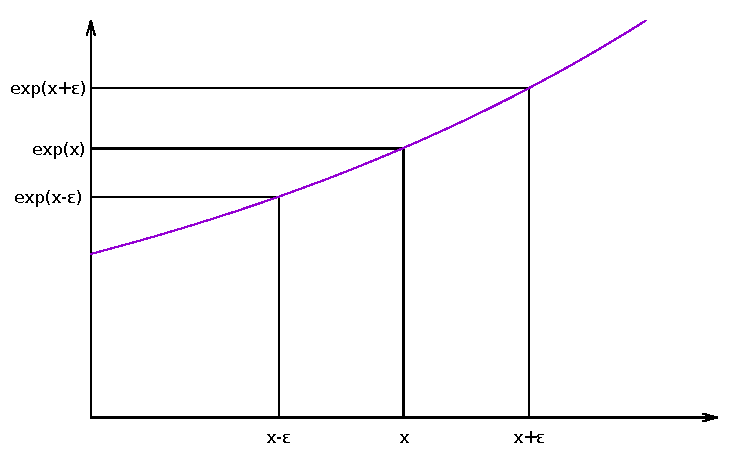
\includegraphics[width=\linewidth]{graphics/exp4.pdf}\label{fig:exp4}
Interval $[x-\varepsilon,x+\varepsilon]$ se nezobrazí na $[e^x-\varepsilon,e^x+\varepsilon]$. Tím pádem $\mathcal{T}^{\mathrm{exp}(x)}(\varepsilon) \neq \mathcal{T}^{\mathrm{exp}(\mathcal{T}^x(\varepsilon))}(\varepsilon)$.
\end{myfigure}

Vidíme, že $|(x-\varepsilon)-x|=|(x+\varepsilon)-x|$, ale $|\mathrm{exp}(x-\varepsilon)-\mathrm{exp}(x)|\neq|\mathrm{exp}(x+\varepsilon)-\mathrm{exp}(x)|$, tedy že přesnost se průchodem nelineární funkcí deformuje a proto se interval $[\mathrm{exp}(x-\varepsilon),\mathrm{exp}(x+\varepsilon)]$ neshoduje s intervalem $[\mathrm{exp}(x)-\varepsilon,\mathrm{exp}(x)+\varepsilon]$. Důsledkem pak je, že nelze rozšířit funkce racionálních čísel na tnumy ve smyslu $\mathcal{T}^{\mathrm{exp}(x)}(\varepsilon) := \mathcal{T}^{\mathrm{exp}(\mathcal{T}^x(\varepsilon)}(\varepsilon)$, ale budeme to muset udělat šetrněji.

Pátráme po metodě, která nám řekne, jak přesné má být číslo na vstupu do funkce, aby jeho obraz byl v zadané přesnosti.

\begin{myfigure}{H}
\caption{Vzor přesnosti před průchodem exponenciálou}
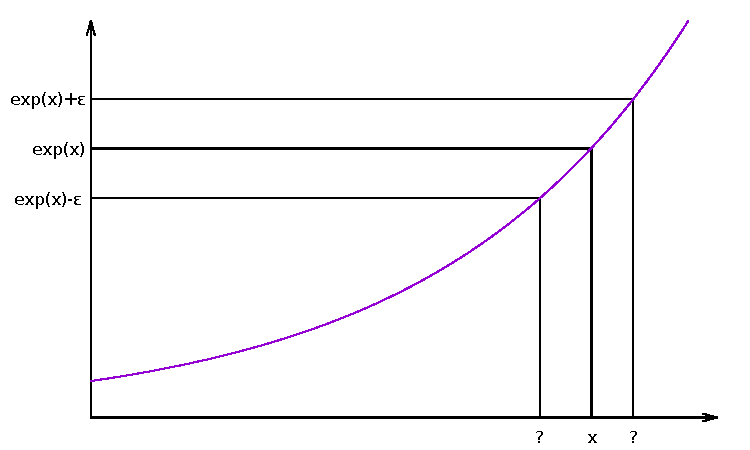
\includegraphics[width=\linewidth]{graphics/exp2.pdf}\label{fig:exp2}
Levý interval je širší než pravý.

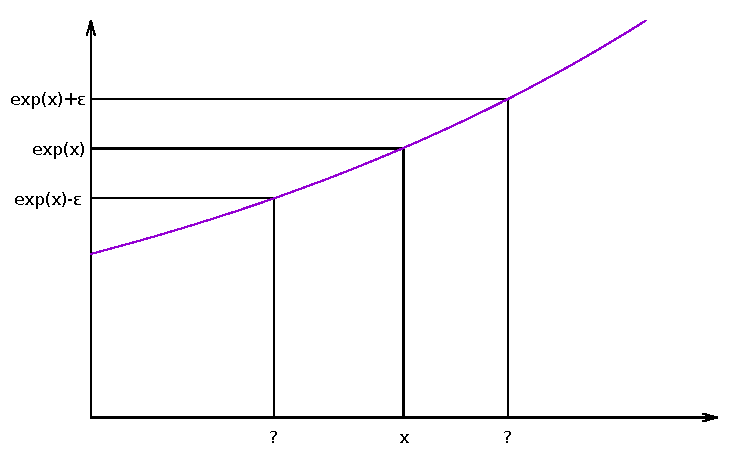
\includegraphics[width=\linewidth]{graphics/exp3.pdf}\label{fig:exp3}
Hledáme, jaké okolí bodu $x$ se zobrazí na $\varepsilon$-okolí bodu $e^x$.
\end{myfigure}

Když si to vyneseme do rovnice, bude vypadat
\begin{equation}\label{invpresexp}
\mathrm{exp}(x)+\varepsilon=\mathrm{exp}(x+w),
\end{equation}
kde hledaná neznámá je $w$.

\begin{myfigure}{H}
\caption{Zobrazení neznámé $w$}
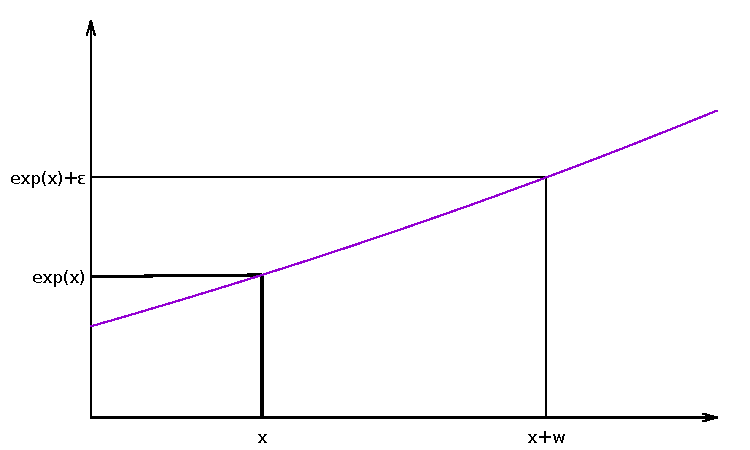
\includegraphics[width=.5\linewidth]{graphics/exp5.pdf}\label{fig:exp5}
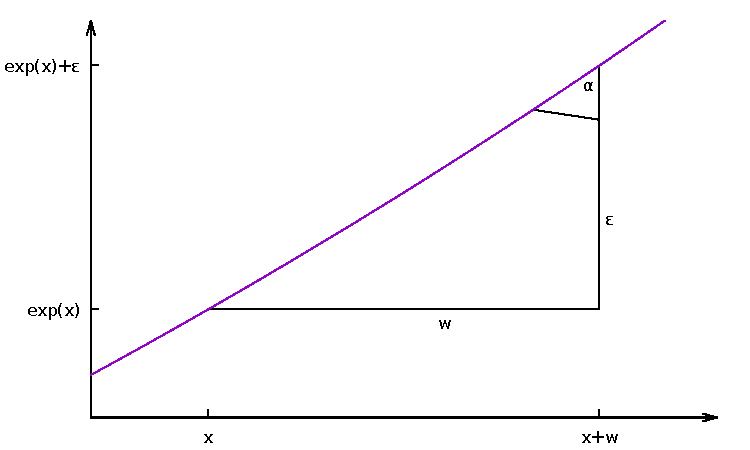
\includegraphics[width=.5\linewidth]{graphics/exp6.pdf}\label{fig:exp6}
Neznámou $w$ lze zobrazit jako jednu z odvěsen, druhá je $\varepsilon$. Fialová čára není přepona, ale exponenciála.
\end{myfigure}

Podívejme se nyní, jaký vztah je mezi $w$ a $\varepsilon$. Pro úhel $\alpha$ při vrcholu $W$ platí, že $\mathrm{ctan}(\alpha) = \frac{\varepsilon}{w}$. Tedy
\begin{equation}
w = \frac{\varepsilon}{\mathrm{ctan}(\alpha)} = \frac{\varepsilon}{\mathrm{tan}(\frac{\pi}{2}-\alpha)} = \frac{\varepsilon}{exp(x+w)}.
\end{equation}

Poslední úprava je přepsání skutečnosti, že tangens je v tomto bodě roven derivaci a derivace exponenciály je exponenciála. Vychází rekurzivní vztah pro $w$, po jeho dosazení do vztahu \ref{invpresexp} dostáváme
\begin{equation}\label{rekpresexp}
\mathrm{exp}(x)+\varepsilon=\mathrm{exp}\left(x+\frac{\varepsilon}{\mathrm{exp}\left(x+\frac{\varepsilon}{\mathrm{exp}(x+\ldots)}\right)}\right).
\end{equation}

Podobným způsobem lze odvodit i vztah pro opačný kraj okolí a to
\begin{equation}\label{rekpresexp2}
\mathrm{exp}(x)-\varepsilon=\mathrm{exp}\left(x-\frac{\varepsilon}{\mathrm{exp}\left(x-\frac{\varepsilon}{\mathrm{exp}(x-\ldots)}\right)}\right),
\end{equation}

dohromady to pak po propojení s notací tnumů dává vztah

\begin{equation}\label{rekpresexp3}
\mathcal{T}^{\mathrm{exp}(x)}(\varepsilon)\in\left[
\mathrm{exp}\left(x-\frac{\varepsilon}{\mathrm{exp}\left(x-\frac{\varepsilon}{\mathrm{exp}(x-\ldots)}\right)}\right), \mathrm{exp}\left(x+\frac{\varepsilon}{\mathrm{exp}\left(x+\frac{\varepsilon}{\mathrm{exp}(x+\ldots)}\right)}\right)\right].
\end{equation}

\begin{myremark}{Obecnější přesnost vzoru}
Odložím si zde obecnější trvzení, které vychází z právě dokázaného vztahu pro exponenciálu, jeho platnost by nyní měla být jasná pro všechny neklesající funkce spojité v $x$.
\begin{lemma}[O přesnosti závislé proměnné]\label{lem:presprom}
\begin{equation}\label{eq:presprom}
f(x)+\varepsilon=f(x+w)\text{,~kde~}w=f\left(x+\frac{\varepsilon}{f^{'}(x+w)}\right).
\end{equation}
\begin{proof}
Tělo důkazu je již v řádcích a obrázcích nad tímto lemmatem. Protože $\varepsilon$ může být jakkoli malé, je úhel $\alpha$ roven derivaci v bodě $x+w$ a proto pak platí právě uvedený vztah.
\end{proof}
\end{lemma}
Rekurzivní vztah vede k nějakému iterativnímu výpočtu, na ten se podíváme v následujících řádcích ohledně exponenciály a logaritmu.
\end{myremark}

Z výše uvedených vztahů by mělo být jasné, že při implementaci budeme hledat pevný bod a proto si zavedeme tzv. \textit{precizní iterátor}.

\begin{definition}[Precizní iterátor exponenciály]
Definujme následující posloupnost:
\begin{equation}
\left[ \mathcal{T}^x\right]_0^{\mathrm{exp},\varepsilon}=\mathcal{T}^{\mathrm{exp}(\mathcal{T}^x(\varepsilon))}(\varepsilon),
\end{equation}
\begin{equation}
\left[ \mathcal{T}^x\right]_{n+1}^{\mathrm{exp},\varepsilon}=\mathcal{T}^{\mathrm{exp}\left(\mathcal{T}^x\left(\frac{\varepsilon}{\left|\left[ \mathcal{T}^x\right]_n^{\mathrm{exp},\varepsilon}\right|+\varepsilon}\right)\right)}(\varepsilon)
\end{equation}
a pokud existuje $m$ tak, že
\begin{equation}
\left[\mathcal{T}^x\right]_m^{\mathrm{exp},\varepsilon} = \left[\mathcal{T}^x\right]_{m+1}^{\mathrm{exp},\varepsilon}\text{, pak klademe}\left[\mathcal{T}^x \right]_\infty^{\mathrm{exp},\varepsilon} := \left[\mathcal{T}^x\right]_m^{\mathrm{exp},\varepsilon}.
\end{equation}
\end{definition}

\begin{consequence}[O exponenciále tnumu]\label{dusl:expotnumu}
Pro tnum $\mathcal{T}^x$ lze najít tnum $\mathcal{T}^{exp(x)}$ a má tvar
\begin{equation}
\mathcal{T}^{exp(x)}(\varepsilon)=\left[\mathcal{T}^x\right]_\infty^{exp,\varepsilon}.
\end{equation}
\begin{proof}
Vychází přímo ze vztahu \ref{rekpresexp3}.
\end{proof}
\end{consequence}

\begin{lispcode}{\texttt{tnum-exp}}{Funkce pro rozšíření funkcí z racionálních čísel na tnumy}
(\textcolor{funkcionalni}{defun} \textcolor{pojmenovan}{tnum-exp} (tnum)
  (\textcolor{funkcionalni}{lambda} (eps)
      (\textcolor{funkcionalni}{loop} \textcolor{obarvi}{for} i \textcolor{obarvi}{from} 0
        \textcolor{obarvi}{for} num = (\textcolor{funkcionalni}{if} (\textcolor{funkcionalni}{zerop} i) (\textcolor{moje}{tnum-to-num} tnum eps) new)
        \textcolor{obarvi}{for} new = (\textcolor{funkcionalni}{if} (\textcolor{funkcionalni}{zerop} i) 1 (\textcolor{funkcionalni}{if} (\textcolor{matematicke}{>} expnum 1) 
          (\textcolor{moje}{tnum-to-num} tnum (\textcolor{matematicke}{/} eps (\textcolor{matematicke}{+} expnum eps))) num))
        \textcolor{obarvi}{for} expnum = (\textcolor{moje}{num-exp} num eps)
        \textcolor{obarvi}{until} (\textcolor{matematicke}{=} num new)
        \textcolor{obarvi}{finally} (\textcolor{funkcionalni}{return} expnum))))
\end{lispcode}

\subsection{Goniometrické}
Goniometrické funkce jsou opět reálné funkce reálné proměnné. Po zkušenosti s implementací exponenciály už nás kód nepřekvapí. První dvě naprogramujeme nízkoúrovňově, zbylé čtyři pak využijí již existujících. Poznamenejme, že $\frac{d}{dx}\mathrm{sin}(x) = \mathrm{cos}(x)$, $\frac{d}{dx}\mathrm{cos}(x) = -\mathrm{sin}(x)$ a že $H(\mathrm{sin}) = [-1,1] = H(\mathrm{cos})$.

\subsubsection{Sinus}
\begin{fact}[Sinus jako Maclaurinova řada \cite{ZDVNNR}]\label{vet:sin_jako_rada}
Funkci $\mathrm{sin}(x)$ lze vyjádřit jako Maclaurinovu řadu ve tvaru
\begin{equation}
\mathrm{sin}(x) =\sum_{i \in \mathbb{N}} (-1)^i \frac{x^{2i+1}}{(2i+1)!} =\frac{x}{1} - \frac{x^3}{3!} + \frac{x^5}{5!} - \frac{x^7}{7!} + \ldots
\end{equation}
Pro důkaz vizte podkapitolu \ref{duk:sin_jako_rada} v příloze \ref{pril:dukazy}.
\end{fact}

Dále protože jsou funkční hodnoty všech možných derivací v intervalu $[-1,1]$, lze Lagrangeův tvar zbytku vyjádřit bez znaménka a pak díky Taylorově větě platí
\begin{equation}
\left|\mathcal{R}^{sin, 0}_n(x)\right|\leq\left|\frac{x^{2n+1+1}}{(2n+1+1)!}\right|=\left|\frac{x^{2n+2}}{(2n+2)!}\right|.
\end{equation}

\begin{consequence}[Sinus numu]
Pro všechna $\varepsilon$ existuje $n\in\mathbb{N}^+$ tak, aby $\left|\frac{x^{2n+2}}{(2n+3)!}\right| \leq \varepsilon$ a pak
\begin{equation}
\mathcal{T}^{\mathrm{sin}(x)}(\varepsilon)=\sum_{i=0}^n (-1)^i \frac{x^{2i+1}}{(2i+1)!}
\end{equation}
\begin{proof}
Běží podobně jako u exponenciály. Jde opět o exponenciálu nad faktoriálem, proto je jasná limita i existence $n$. Dále z omezení $R^{\mathrm{sin}, 0}_n$ lze odvodit $T^{\mathrm{sin}, 0}_n\in[\mathrm{sin}(x)-|R^{\mathrm{sin}, 0}_n|,\mathrm{sin}(x)+|R^{\mathrm{sin}, 0}_n|]$ a pak $T^{\mathrm{sin}, 0}_n\in[\mathrm{sin}(x)-|\frac{x^{2n+2}}{(2n+2)!}|,\mathrm{sin}(x)+|\frac{x^{2n+2}}{(2n+2)!}|]$ a tudíž $T^{\mathrm{sin}, 0}_n\in[\mathrm{sin}(x)-\varepsilon,\mathrm{sin}(x)+\varepsilon]$, z čehož pak $\mathcal{T}^{\mathrm{sin}(x)}(\varepsilon)=T^{\mathrm{sin},0}_n(x)$.
\end{proof}
\end{consequence}

\begin{lispcode}{\texttt{num-sin}}{Funkce pro sinus čísla}
(\textcolor{funkcionalni}{defun} \textcolor{pojmenovan}{num-sin} (x eps)
  (\textcolor{vedlejsi}{let} ((n 0) (result 0) (2n+1 1))
    (\textcolor{funkcionalni}{loop} 
      \textcolor{obarvi}{until} (\textcolor{matematicke}{<=} (\textcolor{matematicke}{abs} (\textcolor{matematicke}{/} (\textcolor{moje}{rat-expt} x (\textcolor{matematicke}{1+} 2n+1))
                        (\textcolor{moje}{factorial} (\textcolor{matematicke}{1+} 2n+1))))
                eps)
      \textcolor{obarvi}{do} (\textcolor{funkcionalni}{progn} 
          (\textcolor{vedlejsi}{incf} result
            (\textcolor{matematicke}{/} (\textcolor{moje}{rat-expt} x 2n+1)
               (\textcolor{moje}{factorial} 2n+1)
               (\textcolor{matematicke}{expt} -1 n)))
          (\textcolor{vedlejsi}{incf} n)
          (\textcolor{vedlejsi}{setf} 2n+1 (\textcolor{matematicke}{1+} (\textcolor{matematicke}{*} 2 n))))
      \textcolor{obarvi}{finally} (\textcolor{funkcionalni}{return} result))))
\end{lispcode}

Protože derivace sinu je kosinus, který nabývá hodnot mezi $-1$ a $1$, nebude nutné provádět korekce přesnosti podle funkční hodnoty derivace a tato skutečnost vede na jednoduchý vztah.

\begin{lemma}[O sinu tnumu]
\begin{equation}
\mathcal{T}^{\mathrm{sin}(x)}(\varepsilon)=\mathcal{T}^{sin(\mathcal{T}^x(\varepsilon))}(\varepsilon)
\end{equation}
\begin{proof}
Plyne nepřímo z lemmatu \ref{lem:presprom} a z omezení absolutních funkčních hodnot kosinu jedničkou. Lemma nelze použít doslovně, protože kosinus není neklesající funkce, ale z argumentu o omezení funkčních hodnot plyne, že nás stejně přesný tvar vzoru přesnosti a tudíž ani bod derivace nezajímá.
\end{proof}
\end{lemma}

\begin{lispcode}{\texttt{tnum-sin}}{Funkce pro sinus tnumu}
(\textcolor{funkcionalni}{defun} \textcolor{pojmenovan}{tnum-sin} (tnum)
  (\textcolor{funkcionalni}{lambda} (eps)
    (\textcolor{moje}{num-sin} (\textcolor{moje}{tnum-to-num} tnum eps) eps)))
\end{lispcode}

\subsubsection{Kosinus}
\begin{fact}[Kosinus jako Maclaurinova řada \cite{ZDVNNR}]\label{vet:cos_jako_rada}
Funkci $\mathrm{cos}(x)$ lze vyjádřit jako Maclaurinovu řadu ve tvaru
\begin{equation}
\mathrm{cos}(x) = \sum_{i\in\mathbb{N}}(-1)^i \frac{x^{2i}}{(2i)!} = \frac{1}{1} - \frac{x^2}{2!} + \frac{x^4}{4!} - \frac{x^6}{6!} + \ldots
\end{equation}
Pro důkaz vizte podkapitolu \ref{duk:cos_jako_rada} v příloze \ref{pril:dukazy}.
\end{fact}

Z Taylorovy věty získáváme omezení Taylorova zbytku
\begin{equation}
|R^{cos}_n(x)|\leq\left|\frac{x^{2n+1}}{(2n+1)!}\right|
\end{equation}
a proto opět hledáme takové $n$, že když pro jakékoli $\varepsilon$ je $|\frac{x^{2n+1}}{(2n+1)!}|\leq\varepsilon$, pak 
\begin{consequence}[Kosinus numu]
\begin{equation}
\mathcal{T}^{\mathrm{cos}(x)}(\varepsilon)=\sum_{i=0}^n(-1)^i \frac{x^{2i}}{(2i)!}.
\end{equation}
\end{consequence}

\begin{lispcode}{\texttt{num-cos}}{Funkce pro výpočet kosinu čísla}
(\textcolor{funkcionalni}{defun} \textcolor{pojmenovan}{num-cos} (x eps)
  (\textcolor{vedlejsi}{let} ((n 0) (result 0) (2n 0))
    (\textcolor{funkcionalni}{loop} 
      \textcolor{obarvi}{until} (\textcolor{matematicke}{<} (\textcolor{matematicke}{abs} (\textcolor{matematicke}{/} (\textcolor{moje}{rat-expt} x (\textcolor{matematicke}{1+} 2n))
                        (\textcolor{moje}{factorial} (\textcolor{matematicke}{1+} 2n))))
                eps)
      \textcolor{obarvi}{do} (\textcolor{funkcionalni}{progn} 
          (\textcolor{vedlejsi}{incf} result
            (\textcolor{matematicke}{/} (\textcolor{moje}{rat-expt} x 2n)
               (\textcolor{moje}{factorial} 2n)
               (\textcolor{matematicke}{expt} -1 n)))
          (\textcolor{vedlejsi}{incf} n)
          (\textcolor{vedlejsi}{setf} 2n (\textcolor{matematicke}{*} 2 n)))
      \textcolor{obarvi}{finally} (\textcolor{funkcionalni}{return} result))))
\end{lispcode}

A nakonec právě naprogramovanou funkci využijeme ke kosinování jakékoli proměnné s tnumem. Postup je stejný jako u sinu a proto už nepíši příslušné lemma a nechávám ho ke zformulování čtenáři.

\begin{lispcode}{\texttt{tnum-cos}}{Funkce pro výpočet kosinu tnumu}
(\textcolor{funkcionalni}{defun} \textcolor{pojmenovan}{tnum-cos} (tnum)
  (\textcolor{funkcionalni}{lambda} (eps)
    (\textcolor{moje}{num-cos} (\textcolor{moje}{tnum-to-num} tnum eps) eps)))
\end{lispcode}

Zbylé goniometrické funkce už naprogramujeme uživatelsky.

\subsubsection{Další goniometrické funkce}
Další goniometrickou funkcí je tangens. Dá se vyjádřit pomocí sinu a kosinu, díky čemuž ho nemusím vyjadřovat jako řadu, i když pro všechny goniometrické funkce řady existují. Nejsou ale konvergentní na celé reálné ose, takže se pro naši knihovnu nehodí.
\begin{fact}[Tangens jako poměr sinu a kosinu \cite{tabulky}]
\begin{equation}
\mathrm{tg}(x)=\frac{\mathrm{sin}(x)}{\mathrm{cos}(x)}
\end{equation}
\end{fact}

\begin{convention}[O vypuštění některých důsledků]
Nyní by měl následovat důsledek že $\mathcal{T}^{\mathrm{tan}(x)}=\mathcal{T}^{\frac{\mathcal{T}^{\mathrm{sin}(x)}}{\mathcal{T}^{\mathrm{cos}(x)}}}$, což je ale myslím jasné a proto zde ani u dalších zřejmých přepsání vzorečků do jazyka tnumů tyto důsledky neuvádím.\hfill$\blacksquare$
\end{convention}

\begin{lispcode}{\texttt{tnum-tan}}{Funkce pro výpočet tangentu tnumu}
(\textcolor{funkcionalni}{defun} \textcolor{pojmenovan}{tnum-tan} (tnum)
  (\textcolor{moje}{tnum/} (\textcolor{moje}{tnum-sin} tnum) (\textcolor{moje}{tnum-cos} tnum)))
\end{lispcode}

Zbylé funkce jsou obrácenou hodnotou již napsaných.

\begin{fact}[Kosekans jako obrácená hodnota sinu \cite{tabulky}]
  \begin{equation}
    \mathrm{csc}(x)=\mathrm{sin}^{-1}(x)
  \end{equation}
\end{fact}
\begin{lispcode}{\texttt{tnum-csc}}{Funkce pro výpočet kosekantu tnumu}
(\textcolor{funkcionalni}{defun} \textcolor{pojmenovan}{tnum-csc} (tnum)
  (\textcolor{moje}{/tnum} (\textcolor{moje}{tnum-sin} tnum)))
\end{lispcode}

\begin{fact}[Sekans jako obrácená hodnota kosinu \cite{tabulky}]
  \begin{equation}
    \mathrm{sec}(x)=\mathrm{cos}^{-1}(x)
  \end{equation}
\end{fact}
\begin{lispcode}{\texttt{tnum-sec}}{Funkce pro výpočet sekantu tnumu}
(\textcolor{funkcionalni}{defun} \textcolor{pojmenovan}{tnum-sec} (tnum)
  (\textcolor{moje}{/tnum} (\textcolor{moje}{tnum-cos} tnum)))
\end{lispcode}

\begin{fact}[Kotangens jako obrácená hodnota tangentu \cite{tabulky}]
  \begin{equation}
    \mathrm{cotg}(x)=tan^{-1}(x)=\frac{\mathrm{cos}(x)}{\mathrm{sin}(x)}
  \end{equation}
\end{fact}
\begin{lispcode}{\texttt{tnum-ctan}}{Funkce pro výpočet kotangentu tnumu}
(\textcolor{funkcionalni}{defun} \textcolor{pojmenovan}{tnum-ctan} (tnum)
  (\textcolor{moje}{tnum/} (\textcolor{moje}{tnum-cos} tnum) (\textcolor{moje}{tnum-sin} tnum)))
\end{lispcode}

\subsection{Logaritmus}
Logaritmus je inverzní funkce k exponenciále. Je opět vyjadřitelná řadou.
\begin{fact}[Logaritmus jako řada \cite{HoMF}]
Pro $x\in\mathbb{R}^+$ platí
  \begin{equation}
    \mathrm{ln}(x)=2\sum_{i\in\mathbb{N}}\frac{1}{2i+1}\left(\frac{x-1}{x+1}\right)^{2i+1}
  \end{equation}
\end{fact}

Člen $\frac{1}{2i+1}(\frac{x-1}{x+1})^{2i+1}$ je menší než $(\frac{x-1}{x+1})^{2i+1}$ a  tento je menší než $(\frac{x-1}{x+1})^{2i}$. Toto je geometrická posloupnost, jejíž $n$-tý zbytek je roven $\frac{(\frac{x-1}{x+1})^{2n+2}}{1-\frac{x-1}{x+1}}$ podle faktu \ref{vet:o_zbytku_geometricke_rady}.
\begin{lispcode}{\texttt{num-ln}}{Funkce pro logaritmus čísla}
(\textcolor{funkcionalni}{defun} \textcolor{pojmenovan}{num-ln} (x eps)
  (\textcolor{vedlejsi}{setf} eps (\textcolor{matematicke}{/} eps 2))
  (\textcolor{vedlejsi}{let} ((n 0) (result 0) (q (\textcolor{matematicke}{/} (\textcolor{matematicke}{1-} x) (\textcolor{matematicke}{1+} x))))
    (\textcolor{funkcionalni}{loop} 
      \textcolor{obarvi}{until} (\textcolor{matematicke}{<=} (\textcolor{matematicke}{/} (\textcolor{matematicke}{expt} q (\textcolor{matematicke}{*} 2 (\textcolor{matematicke}{1+} n))) (\textcolor{matematicke}{-} 1 q))
                eps)
      \textcolor{obarvi}{do} (\textcolor{funkcionalni}{progn} 
          (\textcolor{vedlejsi}{incf} result
            (\textcolor{matematicke}{/} (\textcolor{matematicke}{expt} q (\textcolor{matematicke}{1+} (\textcolor{matematicke}{*} 2 n))) (\textcolor{matematicke}{1+} (\textcolor{matematicke}{*} 2 n))))
          (\textcolor{vedlejsi}{incf} n))
      \textcolor{obarvi}{finally} (\textcolor{funkcionalni}{return} (\textcolor{matematicke}{*} 2 result)))))
\end{lispcode}

Tím bychom měli přirozený logaritmus pro čísla. Podívejme se nyní, jak vypadá omezení nezávislé proměnné pro logaritmus. Po dosazení do vztahu \ref{eq:presprom} získáváme

\begin{equation}
\mathrm{ln}(x)+\varepsilon=\mathrm{ln}\left(x+\frac{\varepsilon}{\mathrm{ln}^{'}(x+w)}\right)
\end{equation}

a protože $\mathrm{ln}(x+w)=(x+w)^{-1}$, pak

\begin{equation}
\mathrm{ln}(x)+\varepsilon=\mathrm{ln}(x+\varepsilon(x+w)),
\end{equation}

tedy násobíme přesnost hodnotou proměnné a protože přesnost nemůže být nulová, použijeme k vyčíslení $\mathcal{T}^x$ nenulový tnum a tím je problém vyřešen. Vezmeme totiž pesimistický odhad $\mathcal{T}^x(\varepsilon_\emptyset)-\varepsilon_\emptyset$ a přenásobíme jím epsilon. Díky třetí podmínce v definici \ref{def:bezpecne_epsilon} toto mohu udělat.

\begin{lispcode}{\texttt{tnum-ln}}{Funkce pro logaritmus tnumu}
(\textcolor{funkcionalni}{defun} \textcolor{pojmenovan}{tnum-ln} (tnum)
  (\textcolor{funkcionalni}{lambda} (eps)
    (\textcolor{matematicke}{multiple-value-bind} (num eps0)
      (\textcolor{moje}{get-nonzero-num+eps} tnum eps)
      (\textcolor{moje}{num-ln} (\textcolor{moje}{tnum-to-num} tnum eps) (\textcolor{matematicke}{*} eps (\textcolor{matematicke}{-} num eps0))))))
\end{lispcode}

\begin{myremark}{Dokončení systému}
Pomocí logaritmu v kombinaci s exponenciálou lze přinést i mocninné operace a ucelím tak základní funkcionalitu knihovny \texttt{tnums}, kterou jsem si předsevzal. Mocninu udělám jako v lemmatu \ref{vet:mocnina_tnumu}.
\begin{lispcode}{\texttt{tnum-expt}}{Funkce pro umonování tnumů}
(\textcolor{funkcionalni}{defun} \textcolor{pojmenovan}{tnum-expt} (tnum1 tnum2)
  (\textcolor{moje}{tnum-exp} (\textcolor{moje}{tnum*} tnum2 (\textcolor{moje}{tnum-ln} tnum1))))
\end{lispcode}

Odmocninu pak píši podle faktu \ref{fac:odmocnina_tnumu}. Oproti mocnině jsou prohozené argumenty, ale tnum-tou odmocninu tnumu chápu tak, že odmocnitel je jako první a odmocněnec jako druhý, říká se \uv{třetí odmocnina z osmi}.

\begin{lispcode}{\texttt{tnum-root}}{Funkce pro odmocňování tnumu}
(\textcolor{funkcionalni}{defun} \textcolor{pojmenovan}{tnum-root} (tnum1 tnum2)
  (\textcolor{moje}{tnum-expt} tnum2 (\textcolor{moje}{/tnum} tnum1)))
\end{lispcode}
\end{myremark}

Takto je tedy dokončena základní funkcionalita knihovny \texttt{tnums} a v další části se podíváme na její používání, perspektivu a doprogramujeme nějaké uživatelské funkce.
\mypart{Rozhraní}
V uživatelské části pojednám o vlastním používání knihovny \texttt{tnums}. Nejprve zkusíme převádět čísla mezi interními reprezentacemi Lispu a tnumů. Poté se podíváme, jak se používají matematické operace a poté spočítáme nějaké matematické funkce. Také ještě několik funkcí doprogramujeme, ale nezávisle na vnitřní implementaci tnumů. Nakonec se podíváme na nedostatky knihovny a její výhled jak v oblasti rozšiřování funkcionality, tak na poli zvyšování efektivity.
\section{Uživatelské funkce}
Uživatelská funkce je funkce, která nezná vnitřní implementaci tnumů (jako funkcí přesnosti) a volá jen funkce rozhraní zobrazené v Tabulce \ref{tab:funkce_rozhrani}. Během programování knihovny již některé mimoděk vznikly (například \texttt{tnum-}), v této kapitole další přidáme. Ukážeme, že síla knihovny spočívá v jednoduchém vytváření nových tnumů a ve velmi silně oddělené vnitřní implementaci od vnějšího chování.

\subsection{Instalace}\label{ssec:inst}
Knihovna \texttt{tnums} je k dostání na githubu na odkaze \url{https://github.com/slavon00/tnums} nebo pro čtenáře tištěné verze na přiloženém fyzickém disku. Je to Lispová knihovna, od uživatele se předpokládá znalost základů práce s Lispem.

Vše, co jsme doposud naprogramovali najdeme v souboru \texttt{src/tnums.lisp} a všechny funkce, které přidáme v této kapitole, pak v \texttt{src/user-functions.lisp}. Testy, které budu ukazovat jsou v souboru \texttt{src/tests.lisp}. Vše je možné jednoduše načíst evaluací souboru \texttt{load.lisp}, jak ukazuje Obrázek \ref{obr:loading}. Při ručním překladu je nutné nejdřív přeložit soubor \texttt{src/tnums.lisp} a až poté \texttt{src/user-}\\\texttt{-functions.lisp}. Pro kompletní obsah adresáře vizte přílohu \ref{pril:adresar}.

Knihovna se v budoucnosti může měnit, takže tyto informace mohou zastarat. Knihovna na githubu bude ale vždy obsahovat soubor \texttt{README.md} nebo ekvivalentní, s popisem postupu instalace.

\begin{myfigure}{H}
\caption{Načtení knihovny \texttt{tnums} do \texttt{SBCL}}
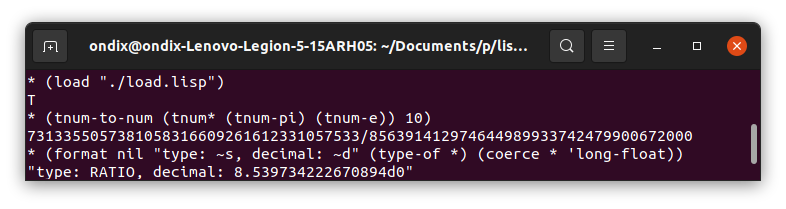
\includegraphics[width=\linewidth]{./graphics/loading2.png}\label{obr:loading}
Aby se nemusely ručně načítat všechny soubory, lze knihovnu \texttt{tnums} též načíst jen evaluací souboru \texttt{load.lisp}. 
\end{myfigure}

\subsection{Převody a konstanty}
Téměř všechny naprogramované funkce berou jako vstup tnumy. To jsou abstraktní struktury (vyjadřující rekurzivní čísla), které interně reprezentujeme jako funkce malých čísel. K vytvoření tnumu z čísla slouží funkce \texttt{num-to-tnum}.

\begin{lisptest}{\texttt{num-to-tnum}}{Představení funkce pro převod $\mathbb{R}\to\mathfrak{T}$}
* (num-to-tnum 42.123)
#<FUNCTION (LAMBDA (EPS) :IN NUM-TO-TNUM) {10020A056B}>
\end{lisptest}

Pro převod opačným směrem slouží inverzní funkce \texttt{tnum-to-num}, která bere tnum a druhý argument představující přesnost, se kterou chceme tnum vyčíslit.

\begin{lisptest}{\texttt{tnum-to-num}}{Představení funkce pro převod $\mathfrak{T}\to\mathbb{Q}$}
* (tnum-to-num * 0.1)
34246/813
\end{lisptest}

Výsledkem vyčíslení je racionální číslo.

\begin{lisptest}{Typ výstupu je číslo}{Ověření typu vraceného numu}
* (type-of *)
RATIO
* (float **)
42.123
\end{lisptest}

Výsledkem vyhodnocení je číslo, které můžeme použít jako vstup do dalších funkcí. Naprogramujme nyní funkci, která bude tnumy převádět na textové řetězce. Takto získáme dlouhé rozvoje v čitelné podobě namísto velkých zlomků.

\begin{lispcode}{\texttt{tnum-to-string}}{Funkce na převod tnumu na textový řetězec}
(\textcolor{funkcionalni}{defun} \textcolor{pojmenovan}{tnum-to-string} (tnum count)
  (\textcolor{vedlejsi}{let} ((num (\textcolor{moje}{tnum-to-num} tnum (\textcolor{matematicke}{1+} count))) (output ""))
    (\textcolor{vedlejsi}{flet} ((get-digit (&optional (end ""))
             (\textcolor{matematicke}{multiple-value-bind} (digit rem) (\textcolor{matematicke}{floor} num)
               (\textcolor{vedlejsi}{setf} output (\textcolor{matematicke}{concatenate} \textquotesingle\textcolor{moje}{string} output 
                                         (\textcolor{funkcionalni}{write-to-string} digit)
                                         end)
                     num (\textcolor{matematicke}{*} 10 rem)))))
      (\textcolor{funkcionalni}{when} (\textcolor{matematicke}{<} num 0) (\textcolor{vedlejsi}{setf} output "-" num (\textcolor{matematicke}{-} num)))
      (\textcolor{moje}{get-digit} ".")  
      (\textcolor{funkcionalni}{dotimes} (i count (\textcolor{matematicke}{concatenate} \textquotesingle\textcolor{moje}{string} output "..."))
        (\textcolor{moje}{get-digit})))))
\end{lispcode}
Funkce bere jako vstup tnum a přirozené číslo značící počet desetinných míst, která má řetězec obsahovat. Otestujeme ji na výpisu Ludolfova čísla.

\begin{lisptest}{\texttt{tnum-string} a \texttt{tnum-pi}}{Vyčíslení Ludolfova čísla na přesnost 50 desetinných míst}
* (tnum-to-string (tnum-pi) 50)
"3.14159265358979323846264338327950288419716939937510..."
\end{lisptest}

Vzhledem k rozšíření množiny přípustných hodnot druhého parametru funkce \texttt{tnum-to-num} mimo $(0,1)$ je možné pohodlně přepínat mezi návratovou hodnotou jako číslem a textovým řetězcem. Ukážeme si to na vyčíslení Eulerova čísla.

\begin{lisptest}{\texttt{tnum-string} a \texttt{tnum-e}}{Vyčíslení Eulerova čísla na přesnost 20 desetinných míst a jeho vrácení jako čísla a jako stringu}
* (tnum-to-num (tnum-e) 20)
611070150698522592097/224800145555521536000
* (tnum-to-string (tnum-e) 20)
"2.71828182845904523536..."
\end{lisptest}

\subsection{Operace}
Operace tnumu je funkce $\bigtimes_{i=0}^{n-1}\mathfrak{T}\rightarrow\mathfrak{T}$, kde $n\in\mathbb{N}$ nazýváme aritou. Operace \texttt{tnum+} a \texttt{tnum*} mohou mít libovolný počet argumentů, operace \texttt{-tnum} a \texttt{/tnum} jsou striktně unární, operace \texttt{tnum-} a \texttt{tnum/} potřebují alespoň jeden argument a operace \texttt{tnum-expt} a \texttt{tnum-root} jsou binární.

V lispu jsou dvě šikovné funkce na inkrementaci a dekrementaci čísla. To samé nyní přidáme pro tnumy.

\begin{lispcode}{\texttt{tnum-1+}}{Funkce pro inkrementaci tnumu o jedničku}
(\textcolor{funkcionalni}{defun} \textcolor{pojmenovan}{tnum-1+} (tnum)
  (\textcolor{moje}{tnum+} (\textcolor{moje}{num-to-tnum} 1) tnum))
\end{lispcode}

Funkce pro dekrementaci se také dá napsat pohodlně uživatelsky.

\begin{lispcode}{\texttt{tnum-1-}}{Funkce pro dekrementaci tnumu o jedničku}
(\textcolor{funkcionalni}{defun} \textcolor{pojmenovan}{tnum-1-} (tnum)
  (\textcolor{moje}{tnum-} tnum (\textcolor{moje}{num-to-tnum} 1)))
\end{lispcode}

Také by šla napsat nejpoužívanější odmocnina a sice druhá.

\begin{lispcode}{\texttt{tnum-sqrt}}{Funkce pro druhou odmocninu tnumu}
(\textcolor{funkcionalni}{defun} \textcolor{pojmenovan}{tnum-sqrt} (tnum)
  (\textcolor{moje}{tnum-root} (\textcolor{moje}{num-to-tnum} 2) tnum))
\end{lispcode}

Výše naprogramované použijeme k zavedení další konstanty, zlatého řezu.

\begin{definition}[Zlatý řez \cite{GR}]
Zlatý řez představuje kladné řešení rovnice \\$x^2-x-1=0$, je tedy roven hodnotě
\begin{equation}
\varphi=\frac{1+\sqrt{5}}{2}.
\end{equation}
\end{definition}

Jedná se o další iracionální konstantu, tentokrát algebraickou, protože je řešením algebraické rovnice a její tnum je jen syntaktický přepis uvedené definice.

\begin{lispcode}{\texttt{tnum-phi}}{Funkce pro tnum Zlatého řezu}
(\textcolor{funkcionalni}{defun} \textcolor{pojmenovan}{tnum-phi} ()
  (\textcolor{moje}{tnum/} (\textcolor{moje}{tnum-1+} (\textcolor{moje}{tnum-sqrt} (\textcolor{moje}{num-to-tnum} 5))) (\textcolor{moje}{num-to-tnum} 2)))
\end{lispcode}

A ještě test.

\begin{lisptest}{\texttt{tnum-phi}}{Představení funkce pro zlatý řez}
* (tnum-to-string (tnum-phi) 50)
"1.61803398874989484820458683436563811772030917980576..."
\end{lisptest}

\subsection{Funkce}
Funkce tnumů jsou všechny unární. Jedná se o přirozený logaritmus, goniometrické funkce a exponenciálu. Omezení definičního oboru jsou stejná jako jsme zvyklí, naprogramované funkce tedy nejsou o nic \uv{slabší}.

Exponenciálu jsme využili už při psaní obecné mocniny. V podobném duchu nyní zavedeme obecný logaritmus. Vyjdeme z faktu, že lze převádět mezi různými základy.

\begin{fact}[Obecný logaritmus jako podíl přirozených  \cite{tabulky}]
Pro $a>1$ a $x\in\mathbb{R}^+$ platí
\begin{equation}
\log_a(x)=\frac{ln(x)}{ln(a)}
\end{equation}
\end{fact}

Nová funkce bude brát dva argumenty, a proto nejde tak úplně o funkci tnumu jak ji v této práci chápeme, ale spíše o matematickou operaci. Nicméně na eleganci zápisu to nic neubírá.

\begin{lispcode}{\texttt{tnum-log}}{Funkce pro výpočet obecného logaritmu}
(\textcolor{funkcionalni}{defun} \textcolor{pojmenovan}{tnum-log} (tnum1 tnum2)
  (\textcolor{moje}{tnum/} (\textcolor{moje}{tnum-ln} tnum2) (\textcolor{moje}{tnum-ln} tnum1)))
\end{lispcode}

Uživatelská funkce potom podobně jako u odmocniny prohazuje argumenty, protože mluvíme vždy o nějakém logaritmu něčeho, například \uv{devítkový logaritmus dvou}. Ten je i předmětem následujícího testu.

\begin{lisptest}{\texttt{tnum-log}}{Vyčíslení devítkového logaritmu dvou}
* (tnum-to-string (tnum-log (num-to-tnum 9) (num-to-tnum 2)) 50)
"0.31546487678572871854976355717138042714979282006594..."
\end{lisptest}

Goniometrické funkce jsou z velké části napsány též uživatelsky, takže by mělo být jasné, jak se s nimi z tohoto pohledu pracuje. Ukážu tedy jen vyčíslení, aby bylo vidět, že funkce opravdu fungují. Následuje výpočet sinu jedničky.

\begin{lisptest}{\texttt{tnum-sin}}{Představení funkce na výpočet sinu tnumu}
* (coerce (tnum-to-num (tnum-sin (num-to-tnum 1)) -20)
    'long-float)
0.8414709848078965d0
\end{lisptest}

\subsection{Rychlost}
Tabulka \ref{tab:rychlost} zobrazuje, jak dlouho běžně trvá vyhodnocení výrazů. Konkrétní hodnoty budou vždy závislé na konkrétním stroji a jeho momentálním zatížení, obecnou představu o časové náročnosti výpočtů však poskytují.

\begin{table}[H]
\begin{mdframed}[backgroundcolor=lightpink,innertopmargin=-2.5pt,innerbottommargin=2.5pt]
\centering
\caption{Doba výpočtů daných výrazů}
\label{tab:rychlost}
\begin{tabular}{| >{\columncolor[gray]{1}} l |>{\columncolor[gray]{1}}p{2.5cm}|}
\hline
\multicolumn{1}{|>{\columncolor[gray]{1}}c|}{Výraz} & Doba vyhodnocení~(s)\\\hline\hline
\texttt{(let ((tn}& \cellcolor[gray]{1} \\
\texttt{~~~~~~(tnum/ (tnum-pi) (tnum-e) (tnum-phi))))} & \multirow{-2}{*}{-}\\ \hline
\texttt{~~~(tnum-to-string tn 50)} & 0.427424 \\ \hline
\texttt{~~~(tnum-to-string (tnum-sin tn) 50)} & 31.412191 \\ \hline
\texttt{~~~(tnum-to-string (tnum-csc tn) 50)} & 4690.939552 \\ \hline
\texttt{~~~(tnum-to-string (tnum-ctan tn) 50))} & 26756.683374 \\ \hline
\end{tabular}

Tabulka v prvním sloupci zobrazuje výrazy, které byly vyhodnocovány, a ve druhém čas, který toto vyhodnocení zabralo. Doba byla měřena makrem \texttt{time} a hodnoty jsou z řádku \uv{(\ldots) seconds of total run time}.
\end{mdframed}
\end{table}

\subsection{Vnější volání}
Rozhraní knihovny \texttt{tnums} -- funkce určené k volání uživatelem -- zobrazuje Tabulka \ref{tab:funkce_rozhrani}.

\begin{table}[H]
\begin{mdframed}[backgroundcolor=lightpink,innertopmargin=-2.5pt,innerbottommargin=2.5pt]
\centering
\caption{Funkce nabízené knihovnou \texttt{tnums}}
\label{tab:funkce_rozhrani}
\begin{tabular}{| >{\columncolor[gray]{1}} c |>{\columncolor[gray]{1}}c|>{\columncolor[gray]{1}}p{4.8cm}|}
\hline
Název & Argumenty & Význam\\ \hline \hline
\texttt{tnum-to-num} & \texttt{tnum:tnum}, \texttt{eps:num} & převod \texttt{tnum}u na číslo s~přesností \texttt{eps}\\
\texttt{tnum-to-string} & \texttt{tnum:tnum}, \texttt{count:num} & převod \texttt{tnum}u na textový řetězec o \texttt{count} desetinných místech\\\hline
\texttt{num-to-tnum}&\texttt{num:num}&převod \texttt{num}u na tnum\\
\texttt{tnum-pi}&$\emptyset$&tnum Ludolfova čísla\\
\texttt{tnum-e}&$\emptyset$&tnum Eulerova čísla\\
\texttt{tnum-phi}&$\emptyset$&tnum Zlatého řezu\\\hline
\texttt{-tnum}&\texttt{tnum:tnum}&$-\texttt{tnum}$\\
\texttt{tnum+}&0+ \texttt{tnum}ů&tnumovský protějšek \texttt{+}\\
\texttt{tnum-}&1+ \texttt{tnum}ů&tnumovský protějšek \texttt{-}\\
\texttt{/tnum}&\texttt{tnum:tnum}&$\texttt{tnum}$\\
\texttt{tnum*}&0+ \texttt{tnum}ů&tnumovský protějšek \texttt{*}\\
\texttt{tnum/}&1+ \texttt{tnum}ů&tnumovský protějšek \texttt{/}\\
\texttt{tnum-expt}&\texttt{arg1:tnum}, \texttt{arg2:tnum}&$\texttt{arg1}^{\texttt{arg2}}$\\
\texttt{tnum-sqrt}&\texttt{arg1:tnum}, \texttt{arg2:tnum}&$\sqrt[\texttt{arg1}]{\texttt{arg2}}$\\
\texttt{tnum-log}&\texttt{arg1:tnum}, \texttt{arg2:tnum}&$\mathrm{log}_{\texttt{arg1}}(\texttt{arg2})$\\
\texttt{tnum-1+}&\texttt{tnum:tnum}&$\texttt{tnum} + 1$\\
\texttt{tnum-1-}&\texttt{tnum:tnum}&$\texttt{tnum} - 1$\\\hline
\texttt{tnum-exp}&\texttt{tnum:tnum}&přirozená mocnina \texttt{tnum}u\\
\texttt{tnum-ln}&\texttt{tnum:tnum}&přirozený logaritmus \texttt{tnum}u\\
\texttt{tnum-sqrt}&\texttt{tnum:tnum}&druhá odmocnina \texttt{tnum}u\\
\texttt{tnum-sin}&\texttt{tnum:tnum}&sinus \texttt{tnum}u\\
\texttt{tnum-cos}&\texttt{tnum:tnum}&kosinus \texttt{tnum}u\\
\texttt{tnum-tan}&\texttt{tnum:tnum}&tangens \texttt{tnum}u\\
\texttt{tnum-csc}&\texttt{tnum:tnum}&kotangens \texttt{tnum}u\\
\texttt{tnum-sec}&\texttt{tnum:tnum}&sekans \texttt{tnum}u\\
\texttt{tnum-ctan}&\texttt{tnum:tnum}&kosekans \texttt{tnum}u\\
\hline\end{tabular}

Tabulka v prvním sloupci zobrazuje funkční symbol, v posledním význam funkce aplikované na argumenty z prostředního sloupce. Čtyři části rozdělené horizontálními čarami jsou po řadě funkce pro převody, konstanty, operace a matematické funkce. Součástí jsou i uživatelské funkce.
\end{mdframed}
\end{table}
\clearpage
\section{Perspektiva}
V bakalářské práci, která se zabývá přesnou reprezentací reálných čísel jsme pochopili, že vše je funkce a funkcionálním paradigmatem implementovali rekurzivní čísla. Vzniklou knihovnu \texttt{tnums} je možné rozvíjet ve smyslu rozšířování funkcionality, zrychlováním výpočtů a opravou chyb.

\subsection{Kontext}
Rekurzivní číslo reprezentujeme jako funkci přesnosti a říkáme mu \textit{tnum}. Současná verze knihovny (\texttt{tnums.3}) je třetí implementací tnumů. Oproti implementaci pomocí řad (\texttt{tnums.1}) je tato reprezentace rychlejší. Oproti implementaci pomocí posloupností (\texttt{tnums.2}) je kód přehlednější.

Implementovali jsme 3 matematické konstanty, obousměrné převody mezi racionálními čísly a tnumy, matematické operace nad tnumy a tnumovské funkce. Operace i funkce kopírují lispovskou syntaxi matematických výrazů.

Implementace je relativně jednoduchá v tom smyslu, že velmi přesně kopíruje matematický jazyk, a tak není moc prostoru pro chyby. Také kód vypadá -- až na výjimku v podobě funkce \texttt{create-list-for-multiplication} -- velmi spořádaně a v základním rozsahu (po začátek části \ref{cast:rozhrani}) ho tvoří jen 169 řádků.

Narozdíl od knihoven představených v kapitole \ref{ssec:knihovny} vrací \texttt{tnums} čísla a nikoli vlastní datové typy. Sice se vytváří abstraktní datové struktury reprezentující čísla, ale výsledky vyčíslení jsou nativního typu \texttt{ratio}. Knihovna tedy nedegraduje na kalkulačku, ale může být přirozeně nasazena v části systému kritické na přesnost. Uživatel je odstíněn od implementace tnumů.

Knihovna toho neumí tolik jako třeba \texttt{mpmath}, naopak umí více než \texttt{computable reals}.

\subsection{Budoucnost}
Funkcionalita knihovny je velmi základní. Pro její rozšíření by bylo možné přidat cyklometrické funkce, další konstanry, případně funkce více proměnných či tetraci.

Dále je možné všechnu funkcionalitu určenou tnumům rozšířit pomocí funkce \texttt{num-to-tnum} i na numy a vytvořit tak přesnou kalkulačku.

Rychlost knihovny odpovídá stručnosti kódu. V kapitole \ref{ssec:optimalizace} jsou navrženy dva směry, kudy by se mohla ubírat optimalizace. V existující reprezentaci 	by se rychlost mohla zvýšit dílčím zapamatováváním proměnných, řádová změna v rychlosti výpočtů bez fundamentálního zásahu do zdrojového kódu ale možná není. Knihovna je relativně pomalá, ale její poslání je přesnost a nikoli rychlost.

\subsection{Problémy}
Při psaní knihovny \texttt{tnums} byl dbán důraz na korektnost. I tak jsou v knihovně lokalizovány dvě chyby, první příliš omezující není, druhá je závažná.

\paragraph{Dotaz na $n$-tou číslici} Pokud řetězec končí řadou číslic $0$ nebo $9$, nemusí být tyto a jedna předcházející číslice správně. Číslo sice správně je ($2.999...=3$), ale číslice bez kontextu správně nejsou.
\begin{lisptest}{Rozvoj $\sqrt{9}$}{Číslo 3 lze zapsat jako číslo \uv{$2.999\ldots$}}
* (tnum-to-string (tnum-sqrt (num-to-tnum 9)) 50)
"2.99999999999999999999999999999999999999999999999999..."
\end{lisptest}

\paragraph{Odmocnina čísla $\leq 1$}
Knihovna vrací správně odmocniny jen čísel větších než jedna.
\begin{lisptest}{$\sqrt{1}$}{Při volání odmocniny čísla jedna se místo jedničky vrací Eulerovo číslo}
* (tnum-to-string (tnum-sqrt (num-to-tnum 1)) 50)
"2.71828182845904523536028747135266249775724709369995..."
\end{lisptest}

\subsection{Optimalizace}\label{ssec:optimalizace}
Jak jsme viděli v Tabulce \ref{tab:rychlost}, vyčíslení tnumu nemusí být dílem okamžiku, ale může trvat i velmi dlouho. Existují nejméně dva směry, kudy by se mohla ubírat optimalizace pro zrychlení výpočtů čísel s libovolnou přesností -- paralelizace a databáze.

\subsubsection{Paralelizace}
Všechen napsaný kód je sekvenční. Když vyčíslujeme \texttt{tnum-pi}, po vypočtení prvního členu se jde na další, ten se přičte a takto se to opakuje až po ukončení cyklu. Rychlejší by bylo, pokud by jeden proces byl zodpovědný pouze za sčítání řady a jednotlivé členy sčítané posloupnosti delegoval na výpočet jiným procesům. Celý výpočet by pak nemusel běžet jen v jednom procesu, na jednom jádře. To stejné platí u funkcí.

Dalším vhodným místem pro použití paralelizace je funkce \texttt{tnum+}. Ta sčítá namapovaný seznam tnumů a mapování by mohlo probíhat paralelně, jednotlivé výsledky mohou přijít v různých časech a hlavní vlákno by se staralo jen o vytvoření výsledného seznamu. Výpočet jednotlivých členů by mohl běžet pro každý člen zvlášť, ve vlastním procesu.

Další vhodné místo je funkce \texttt{create-list-for-multiplication}, která také vrací seznam. Jde o seznam čísel, která byla nezávisle na ostatních vypočtena funkcí \texttt{tnum-to-num}. Tyto výpočty mohou opět vykonávat paralelní procesy, je to tedy vhodné místo pro nasazení paralelizace.

\subsubsection{Databáze}
Druhým podstatným vylepšením by bylo vytvoření nástroje pro přístup k již vypočteným výsledkům. Při pokusu o vyčíslení tnumu dojde k dotazu na tnum a přesnost a při schodě se výsledek vrátí. Jinak se tnum vypočte, uloží a vrátí.

Otázek s tímto zlepšením je několik:
\begin{itemize}
\item{Jak ukládat tnumy?}
\item{Jak zabránit, aby nám někdo nahrával chybné výsledky?}
\item{Je morální užívat výsledků, za které zaplatil strojovým časem někdo jiný?}
\end{itemize}

Lepší by bylo, kdyby se na výpočet dalo navazovat. Pak by se nemusel každý výsledek bez záznamu počítat odznova, ale jen od nejbližší horší přesnosti.

Další problém je, jak ukládat tnumy do databáze. Mohly by to být textové řetězce.

I zde je prostor pro urychlení některých výpočtů. Například pokud bude dotaz mířit na číslo opačné k číslu, které v databázi záznam má, může se použít tento záznam a jen změnit znaménko.

Největší výzvu představuje odhalování ekvivalencí tnumů. Pokud je dotaz mířen na tnum, jehož ekvivalent již v systému máme, lze vrátit tento. Triviální je sčítání s nulou, násobení a mocnění jedničkou. Další ekvivalence tnumů už může být mnohem skrytější. Číslo $x^3$ lze napsat jako $x*x*x$. Číslo $x*3$ lze napsat jako $x+x+x$. To už nejsou tak triviální vztahy a přitom jejich souvislost může vést k mnohem rychlejším výpočtům. A že platí rovnost $4*\sum_{i\in\mathbb{N}}\frac{(-1)^i}{2i+1}=\pi=\sum_{i\in\mathbb{N}}\frac{1}{16^i}(\frac{4}{8i+1}-\frac{2}{8i+4}-\frac{1}{8i+5}-\frac{1}{8i+6})$? To už je velmi složité.

\subsection{Adekvátnost} V kapitole \ref{kap:predstava} bylo zadáno 6 podmínek, které musí abstraktní struktury splňovat. Tnumy všechny tyto podmínky dodržují:
\begin{itemize}
\item{vyčíslování tnumů zajišťuje funkce \texttt{tnum-to-num},}
\item{přesnost zajišťuje samotná podstata tnumů jako funkcí přesnosti,}
\item{matematické operace tnumy podporují,}
\item{matematické funkce tnumy podporují,}
\item{tnumy lze vracet jako výsledky funkcí,}
\item{tnumy lze použít jako argumenty funkcí.}
\end{itemize}
Tnumy tak splňují podmínky na abstraktní datové struktury. Tnumy jsou adekvátní pro realizaci přesných výpočtů s reálnými čísly.
\begin{kiconclusions}
Popsal jsem, jak jsou vytvořena přirozená čísla pomocí teorie množin, také jak na tomto základě vznikají další číselné obory. Dále jsem popsal, jak se s \textbf{čísly} pracuje v paměti v počítače.

Také bylo zmíněno, že číselná osa je tvořena \textbf{reálnými čísly} a pokud použijeme více os, dostáváme strukturovaná čísla. Zamysleli jsme se, jestli jsou všechna reálná čísla rekurzivní a bohužel jsme dostali negativní odpověď.

Představil jsem, jak vypadají \textbf{výpočty s reálnými čísly}. Kromě matematických operací to byly matematické funkce. Zjistili jsme, že všechny tyto výpočty, včetně samotných reálných konstant lze reprezentovat jako funkce.

V textu jsme se věnovali i produktu celého tohoto snažení a sice programování Lispovské knihovny \texttt{tnums} implementující \textbf{přesné výpočty s reálnými čísly}. Také jsem přinesl několik příkladů, jak uživatelsky funkcionalitu rozšiřovat.
\end{kiconclusions}
\begin{kiconclusions}[english]
I have described how natural numbers are created using set theory, as well as on this basis, other numerical fields are created. I also described how to deal with \textbf{numbers} in memory of a computer.

It was also mentioned that the numerical axis is made up of \textbf{real numbers} and if we use more axes, we get structured numbers. We wondered if all real numbers are computable and unfortunately we got a negative answer.

I introduced what \textbf{real numbers' computation} looks like. In addition to mathematical operations there were mathematical functions. We found that all these calculations, including the real constants themselves, can be represented as functions.

In the text, we also focused on the product of all this effort, namely programming Lisp \texttt{tnums} library implementing \textbf{precise real numbers' computation}.

I also brought some examples of how user can extend functionality.
\end{kiconclusions}
\clearpage
\printbibliography[heading=bibintoc, title={Seznam literatury}]
\appendix
\section{Některé důkazy}\label{pril:dukazy}
Zde uvedu některé důkazy, které jsou mimo těžiště práce a pro pochopení práce s tnumy nejsou zapotřebí. Nějaké zájemce by ale mohlo zajímat, jak se některé důkazy vedou a ikdyž se nehodí je napsat přímo v textu práce, zde mohou být.
\subsection{Fakt \ref{vet:o_castecnem_souctu_geometricke_rady} -- O částečném součtu geometrické řady}\label{duk:o_castecnem_souctu_geometricke_rady}
\begin{proof}
Částečný součet je z definice $s^a_n=a+aq+\ldots+aq^n$. Užitím vztahu
\begin{equation}
(1-q)(1+q+q^2+\ldots+q^n)=(1-q)^{n+1}
\end{equation}
dostaneme
\begin{equation}
s^a_n=a(1+q+q^2+\ldots+q^n)=a\frac{1-q^{n+1}}{1-q}.
\end{equation}
\end{proof}

\subsection{Fakt \ref{vet:o_geometricke_rade} -- O geometrické řadě}\label{duk:o_geometricke_rade}
\begin{proof}
Po užití limity na obě strany ze lemmatu \ref{vet:o_castecnem_souctu_geometricke_rady} dostáváme 
\begin{equation}
\sum_{i\in\mathbb{N}}aq^i=\lim_{n\to\infty}s^a_n=\lim_{n\to\infty}a\frac{1-q^{n+1}}{1-q}=\frac{a}{1-q}.
\end{equation}
\end{proof}

\subsection{Fakt \ref{vet:o_zbytku_geometricke_rady} -- O zbytku geometrické řady}\label{duk:o_zbytku_geometricke_rady}	
\begin{proof}
\begin{equation}
R_n = \sum_{i\in\mathbb{N}}aq^i -s^a_n =\frac{a}{1-q} - a\frac{1-q^{n+1}}{1-q} = \frac{a-a+aq^{n+1}}{1-q} = \frac{aq^{n+1}}{1-q}
\end{equation}
\end{proof}

\subsection{Fakt \ref{vet:exp_jako_rada} -- O exponenciále jako Maclaurinově řadě}\label{duk:exp_jako_rada}
\begin{proof}
\begin{equation}
\begin{split}
e^x = \sum_{i\in\mathbb{N}}\frac{exp^{(i)}(0)}{i!}x^i = \left[\begin{matrix}\frac{d}{dx} exp(x) = exp(x) \\ \end{matrix}\right] = \frac{exp(0)}{1} + \frac{exp(0)}{1}x +\\ +\frac{exp(0)}{2}x^2 + \ldots= \left[\begin{matrix} exp(0)=1 \end{matrix}\right] = \frac{1}{1} + \frac{x}{1} + \frac{x^2}{2} + \ldots=\sum_{i\in\mathbb{N}}\frac{x^i}{i!}
\end{split}
\end{equation}
\end{proof}

\subsection{Fakt \ref{vet:sin_jako_rada} -- O sinu jako Maclaurinově řadě}\label{duk:sin_jako_rada}
\begin{proof}
\begin{equation}
\begin{split}
sin(x)=\sum_{i\in\mathbb{N}}\frac{sin^{(i)}(0)}{i!}x^i=\left[\begin{matrix}\frac{d}{dx} sin(x)=cos(x) \\ \frac{d}{dx} cos(x)=-sin(x) \end{matrix} \right] =\\= \frac{sin(0)}{1} + \frac{cos(0)}{1}x-\frac{sin(0)}{2}x^2-\frac{cos(0)}{6}x^3+\frac{sin(0)}{24}x^4+\frac{cos(0)}{120}x^5\ldots=\\=\left[\begin{matrix} sin(0)=0\\ cos(0)=1 \end{matrix}\right]=\frac{x}{1}-\frac{x^3}{6}+\frac{x^5}{120}+\ldots=\sum_{i\in\mathbb{N}}(-1)^i\frac{x^{2i+1}}{(2i+1)!}
\end{split}
\end{equation}
\end{proof}

\subsection{Fakt \ref{vet:cos_jako_rada} -- O kosinu jako Maclaurinově řadě}\label{duk:cos_jako_rada}
\begin{proof}
\begin{equation}
\begin{split}
cos(x)=\sum_{i\in\mathbb{N}}\frac{cos^{(i)}(0)}{i!}x^i=\left[\begin{matrix}\frac{d}{dx} cos(x)=-sin(x) \\ \frac{d}{dx} sin(x)=cos(x) \end{matrix} \right] = \\ =\frac{cos(0)}{1} - \frac{sin(0)}{1}x - \frac{cos(0)}{2}x^2+\frac{sin(0)}{6}x^3+\frac{cos(0)}{24}x^4\ldots=\\=\left[\begin{matrix} cos(0)=1 \\ sin(0)=0 \end{matrix}\right]=\frac{1}{1}-\frac{x^2}{2}+\frac{x^4}{24}+\ldots=\sum_{i\in\mathbb{N}}(-1)^i\frac{x^{2i}}{(2i)!}
\end{split}
\end{equation}
\end{proof}

\clearpage
\section{Obsah přiloženého CD/DVD}\label{pril:adresar}
Na samotném konci textu práce je uveden stručný popis obsahu
přiloženého CD/DVD, tj.~jeho závazné adresářové struktury, důležitých
souborů apod.

\begin{description}
\item[\texttt{doc/}] \hfill \\
Adresář se soubory
\begin{itemize}
\item{\texttt{OndrejSlavikBP.pdf} -- tento text ve formátu PDF a}
\item{\texttt{bak/} -- adresář se všemi soubory pro vysázení tohoto textu, stačí dvakrát přeložit \texttt{PDFLaTex}em.}
\end{itemize}

\item[\texttt{load.lisp}] \hfill \\
Přeložením tohoto souboru ve vašem oblíbeném interpretu/kompilátoru Lispu získáte plnou funkcionalitu knihovny \texttt{tnums}, kterou jsme právě doprogramovali. Načítá soubory \texttt{src/tnums.lisp} a \texttt{src/user-functions.lisp}.

\item[\texttt{src/}] \hfill \\
Adresář se soubory
\begin{itemize}
\item{\texttt{tnums.lisp} -- základ knihovny z části 2 této práce,}
\item{\texttt{user-function.lisp} -- rozšíření knihovny o vědomě uživatelské funkce ze šesté kapitoly a}
\item{\texttt{tests.lisp} -- zakomentované výrazy, které zde byly popsány jako Lispový test i s výsledky, na které se vyhodnotí.}
\end{itemize}

\item[\texttt{README.md}] \hfill \\
Soubor představující knihovnu \texttt{tnums} a obsahující i několik příkladů výpočtů, které podporuje. Součástí je i kapitola o načtení knihovny evaluací souboru \texttt{load.lisp}, nejedná se tedy o instalaci v pravém slova smyslu.

\item[\texttt{install/}] \hfill \\
Adresář se soubory
\begin{itemize}
\item{\texttt{sbcl-2.1.6-source.tar.bz2} -- intalátor SBCL, konzolového kompilátoru ANSI Common Lispu,}
\item{\texttt{code-1.57.1-1623937013-amd64.deb} -- instalátor VS code, rozšiřitelného textového editoru a}
\item{\texttt{2gua.rainbow-brackets-0.0.6.vsix} -- instalátor rozšíření Rainbow Brackets pro přehledné obarvování závorek.}
\end{itemize}

\item[\texttt{LISENCE}] \hfill \\
Licenší soubor -- knihovna je publikována pod GNU GPLv3.
\end{description}

\end{document}